\mfpicnumber{1}

\opengraphsfile{QuadraticFunctions}

\setcounter{footnote}{0}

\label{QuadraticFunctions}

\subsection{Graphs of Quadratic Functions}
\label{GraphsofQuadraticFunctions}


You may recall studying quadratic equations in a previous Algebra course.  If not, you may wish to refer to Section \ref{AppQuadEqus} to revisit this topic. In this section, we review those equations in the context of our next family of functions: the quadratic functions.

\medskip

\colorbox{ResultColor}{\bbm

\begin{defn}[Quadratic Function] \label{quadraticfunction} A\index{function ! quadratic}\index{quadratic function ! definition of} \textbf{quadratic function} is a function of the form \[ f(x) = ax^2 + bx + c,\] where $a$, $b$ and $c$ are real numbers with $a \neq 0$.  The domain of a quadratic function is $(-\infty, \infty)$.

\end{defn}

\ebm}

\medskip

As in Definitions \ref{constantfunction} and \ref{linearfunction}, the independent variable in Definition \ref{quadraticfunction} is $x$ while the  values $a$, $b$ and $c$ are parameters. Note that $a \neq 0$ - otherwise we would have a linear function (see Definition  \ref{linearfunction}).

\medskip

The most basic quadratic function is $f(x) = x^2$, the squaring function, whose graph appears below along with a corresponding table of values. Its shape may look familiar from your previous studies in Algebra -- it is called a \index{parabola ! graph of a quadratic function} \textbf{parabola}. The point $(0,0)$ is called the\index{parabola ! vertex}\index{vertex ! of a parabola} \textbf{vertex} of the parabola because it is the sole point where the function obtains its extreme value, in this case, a minimum of $0$ when $x = 0$. 

\medskip

Indeed, the range of $f(x) = x^2$ appears to be $[0, \infty)$ from the graph. We can substantiate this algebraically since for all $x$, $f(x) = x^2 \geq 0$.  This tells us that the range of $f$ is a subset of $[0, \infty)$.  To show that the range of $f$ actually \text{equals} $[0, \infty)$, we need to show that every real number $c$ in $[0, \infty)$ is in the range of $f$.  That is, for every $c \geq 0$, we have to show $c$ is an output from $f$.  In other words, we have to show there is a real number $x$ so that  $f(x) = x^2 = c$.  Choosing $x = \sqrt{c}$, we find $f(x) = f(\sqrt{c}) = (\sqrt{c})^2 = c$, as required.\footnote{This assumes, of course, $\sqrt{c}$ is a real number for all real numbers $c \geq 0$ \ldots} 

\medskip

\begin{center}

\setlength\columnsep{-10pt}
\begin{multicols}{2}

$\begin{array}{|c||c|}  \hline

x &f(x) = x^2 \\ \hline
 -2 & 4  \\  \hline
-\frac{3}{2} & \frac{9}{4} \vphantom{\frac{1}{1_{Y}}} \\ \hline
 -1 & 1  \\  \hline
 0  & 0  \\  \hline
 1 &  1 \\  \hline
\frac{3}{2} & \frac{9}{4} \vphantom{\frac{1}{1_{Y}}} \\ \hline
 2 & 4  \\  \hline

\end{array}$

\columnbreak

\begin{mfpic}[20]{-3}{3}{0}{5.5}

\axes
\tlabel[cc](-3,4){\scriptsize $(-2,4)$}
\tlabel[cc](-2.5,2.25){\scriptsize $\left(-\frac{3}{2},\frac{9}{4}\right)$}
\tlabel[cc](-2,1){\scriptsize $(-1,1)$}
\tlabel[cc](0,-0.5){\scriptsize $(0,0)$}
\tlabel[cc](1.75,1){\scriptsize $(1,1)$}
\tlabel[cc](2.25,2.25){\scriptsize $\left(\frac{3}{2},\frac{9}{4}\right)$}
\tlabel[cc](2.75,4){\scriptsize $(2,4)$}
\tlabel[cc](3,-0.5){\scriptsize $x$}
\tlabel[cc](0.5,5.5){\scriptsize $y$}
\xmarks{-2,-1,1,2}
\ymarks{1,2,3,4}
\tcaption{$f(x) = x^2$}
\tlpointsep{4pt}
\axislabels {x}{{\scriptsize $-2 \hspace{7pt}$} -2, {\scriptsize $-1 \hspace{7pt}$} -1, {\scriptsize $1$} 1, {\scriptsize $2$} 2}
\axislabels {y}{{\scriptsize $1$} 1, {\scriptsize $2$} 2, {\scriptsize $3$} 3, {\scriptsize $4$} 4}
\penwd{1.25pt}
\arrow \reverse \arrow \function{-2.2,2.2,0.1}{x**2}
\point[4pt]{(-2,4), (-1.5,2.25), (-1,1), (0,0), (1,1), (1.5,2.25), (2,4)}
\end{mfpic}  \\

\end{multicols}
\setlength\columnsep{10pt}

\end{center}

\medskip

\co{The techniques we used to graph many of the absolute value functions in Section \ref{AbsoluteValueFunctions} can be applied to quadratic functions, too.  In fact, k}Knowing the graph of $f(x) = x^2$ enables us to graph \emph{every} quadratic function, but there's some extra work involved.  We start with the following theorem:

\medskip

\colorbox{ResultColor}{\bbm

\begin{thm}  \label{standardformgraph}  For real numbers $a$, $h$ and $k$ with $a\neq 0$, the graph of  $F(x) = a(x-h)^2 + k$ is a parabola with vertex $(h,k)$.  If $a>0$, the graph resembles  `$\smile$.'  If $a<0$, the graph resembles `$\frown$.'  Moreover, the vertical line $x=h$ is the \index{axis of symmetry ! quadratic function} \textbf{axis of symmetry} of the graph of $y = F(x)$.
\end{thm}
\ebm}

\medskip

\co{To prove Theorem \ref{standardformgraph} the reader is encouraged to revisit the discussion following the proof of Theorem \ref{linearabsvaluegraphs}, replacing every occurrence of absolute value notation with the squared exponent.\footnote{i.e., replace $|x|$ with $x^2$, $|c|$ with $c^2$, $|x-h|$ with $(x-h)^2$.} Alternatively, the reader can skip ahead and read the statement and proof of Theorem \ref{linearmononialgraphs} in Section \ref{GraphsofPolynomials}.  In the meantime we put Theorem \ref{standardformgraph}  to good use in the next example.}

\begin{ex} \label{parabolaex1} $~$


\begin{enumerate}

\item  Graph the following functions using Theorem \ref{standardformgraph}. Find the vertex, zeros and axis-intercepts (if any exist). Find the extrema and then list the intervals over which the function is increasing, decreasing or constant.

\begin{multicols}{2}
\begin{enumerate}

\item  $f(x) = \dfrac{(x-3)^2}{2}$ 

\item  $g(x) = (x+2)^2 - 3$ \vphantom{$f(x) = \dfrac{(x-3)^2}{2}$}

\setcounter{HW}{\value{enumii}}
\end{enumerate}
\end{multicols}

\begin{multicols}{2}
\begin{enumerate}
\setcounter{enumii}{\value{HW}}

\item  $h(t) = -2(t-3)^2+1$ \vphantom{$\dfrac{(3-2t)^2 +1}{2}$}

\item  $i(t) = \dfrac{(3-2t)^2 +1}{2}$ 
\end{enumerate}
\end{multicols}

\item  Use Theorem \ref{standardformgraph} to write a possible formula for $H(x)$  whose graph is given below:

\begin{center}

\begin{mfpic}[20]{-3}{3}{-3}{4}
\axes
\tlabel[cc](3,-0.5){\scriptsize $x$}
\tlabel[cc](0.5,4){\scriptsize $y$}
\xmarks{2,-1, 1, 2}
\ymarks{-2,-1,1,2,3,4}
\tcaption{\scriptsize $y=H(x)$}
\tlpointsep{4pt}
\scriptsize
\tlabel[cc](-1.25, 1){$(0,1)$}
\tlabel[cc](1, 3.5){$(1,3)$}
\axislabels {x}{{$-2 \hspace{7pt}$} -2,   {$-1 \hspace{7pt}$} -1, {$1$} 1, {$2$} 2}
\axislabels {y}{{$-2$} -2, {$2$} 2, {$3$} 3}
\normalsize
\penwd{1.25pt}
\arrow \reverse \arrow \function{-0.73,2.73,0.1}{(-2)*((x-1)**2)+3}
\point[4pt]{(0,1), (1,3)}
\end{mfpic}

\end{center}

\end{enumerate}

\vspace*{-.15in}

\enlargethispage{.1in}

{\bf Solution.}

\begin{enumerate}

\item

\begin{enumerate}

\item For $f(x) = \frac{(x-3)^2}{2}  = \frac{1}{2} (x-3)^2+0$, we identify $a = \frac{1}{2}$, $h = 3$ and $k = 0$.  Thus the vertex is $(3,0)$ and the parabola opens upwards.  The only $x$-intercept is $(3,0)$.  Since $f(0) = \frac{1}{2} (0-3)^2 = \frac{9}{2}$, our $y$-intercept is $\left(0, \frac{9}{2}\right)$.  To help us graph the function, it would be nice to have a third point and we'll use symmetry to find it.  The $y$-value three units to the \textit{left} of the vertex is $4.5$, so the $y$-value must be $4.5$ three units to the \textit{right} of the vertex as well.  Hence, we have our third point:  $\left(6, \frac{9}{2}\right)$.  From the graph, we get that the range is $[0, \infty)$ and see that $f$ has the minimum value of $0$ at $x = 3$ and no maximum.  Also, $f$ is decreasing on $(-\infty, 3]$ and increasing on $[3, \infty)$.  The graph is the one on the left of the two on the next page.

\item For $g(x) = (x+2)^2 - 3 = (1)(x-(-2))^2+(-3)$, we identify $a = 1$, $h = -2$ and $k = -3$.  This means that the vertex is $(-2,-3)$ and the parabola opens upwards.  Thus we have two $x$-intercepts. To find them, we set $y = g(x) = 0$ and solve.  Doing so yields the equation $(x+2)^2 - 3 = 0$, or $(x+2)^2 = 3$.  Extracting square roots gives us the two zeros of $g$:  $x + 2 = \pm \sqrt{3}$, or $x = -2 \pm \sqrt{3}$.  Our $x$-intercepts are $(-2-\sqrt{3}, 0) \approx (-3.73, 0)$ and $(-2+\sqrt{3}, 0) \approx (-0.27, 0)$.  We find $g(0) = (0+2)^2-3 = 1$ so our $y$-intercept is $(0,1)$.  Using symmetry, we get $(-4,1)$ as another point to help us graph.  The range of $g$ is $[-3, \infty)$.  The minimum of $g$ is $-3$ at $x = -2$, and $g$ has no maximum. Moreover, $g$ is decreasing on $(-\infty, -2]$ and $g$ is increasing on $[-2, \infty)$.  The graph is below on the right.

\begin{center}

\begin{multicols}{2}

\begin{mfpic}[15]{-1}{7}{-1}{6}
\axes
\tlabel[cc](-1,4.5){\scriptsize $(0,4.5)$}
\tlabel[cc](3,-0.5){\scriptsize $(3,0)$}
\tlabel[cc](7,4.5){\scriptsize $(6,4.5)$}
\tlabel[cc](7,-0.5){\scriptsize $x$}
\tlabel[cc](0.5,6){\scriptsize $y$}
\xmarks{1,2,4,5,6}
\ymarks{1,2,3,4,5}
\tcaption{\scriptsize $f(x) =\frac{(x-3)^2}{2}$}
\tlpointsep{4pt}
\axislabels {x}{{\scriptsize $1$} 1,{\scriptsize $2$} 2, {\scriptsize $4$} 4,{\scriptsize $5$} 5,{\scriptsize $6$} 6}
\axislabels {y}{{\scriptsize $1$} 1,{\scriptsize $2$} 2,{\scriptsize $3$} 3,{\scriptsize $4$} 4}
\penwd{1.25pt}
\arrow \reverse \arrow \function{-0.4,6.4,0.1}{((x-3)**2)/2}
\point[4pt]{(0, 4.5), (3,0), (6,4.5)}
\end{mfpic}

\begin{mfpic}[18]{-5}{1}{-3}{2.5}
\axes
\tlabel[cc](-5,1){\scriptsize $(-4,1)$}
\tlabel[cc](-2,-3.5){\scriptsize $(-2,-3)$}
\tlabel[cc](0.75,1){\scriptsize $(0,1)$}
\tlabel[cc](1,-0.5){\scriptsize $x$}
\tlabel[cc](0.5,2.5){\scriptsize $y$}
\xmarks{-4,-3,-2,-1}
\ymarks{-3,-1,1}
\tcaption{\scriptsize $g(x) =(x+2)^2-3$ \vphantom{$f(x) =\frac{(x-3)^2}{2}$}}
\tlpointsep{4pt}
\axislabels {x}{{\scriptsize $-4 \hspace{7pt}$} -4,{\scriptsize $-3 \hspace{7pt}$} -3,{\scriptsize $-2 \hspace{7pt}$} -2, {\scriptsize $-1 \hspace{7pt}$} -1}
\axislabels {y}{{\scriptsize $-3$} -3,{\scriptsize $-1$} -1,{\scriptsize $-2$} -2,{\scriptsize $1$} 1}
\penwd{1.25pt}
\arrow \reverse \arrow \function{-4.2,0.2,0.1}{((x+2)**2)-3}
\point[4pt]{(-4,1), (-3.73, 0), (-2,-3),  (-0.27, 0), (0,1)}
\end{mfpic}  

\end{multicols}

\end{center}

\item   Given $h(t) = -2(t-3)^2+1$, we identify $a = -2$, $h = 3$ and $k = 1$.  Hence the vertex of the graph is $(3,1)$ and the parabola opens downwards.   Solving $h(t) =-2(t-3)^2+1 = 0$ gives $(t-3)^2 = \frac{1}{2}$.  Extracting square roots\footnote{and rationalizing denominators!} gives $t - 3 = \pm \frac{\sqrt{2}}{2}$, so that when we add $3$ to each side,\footnote{and get common denominators!} we get $t = \frac{6 \pm \sqrt{2}}{2}$.  Hence, our $t$-intercepts are $\left(\frac{6 - \sqrt{2}}{2}, 0 \right) \approx (2.29, 0)$ and $\left(\frac{6 + \sqrt{2}}{2}, 0 \right) \approx (3.71, 0)$. To find the $y$-intercept, we compute $h(0) = -2(0-3)^2+1 = -17$. Thus the $y$-intercept is $(0,-17)$.  Using symmetry, we also have that $(6,-17)$ is on the graph which we show on the left side at the top of the next page.

\item  We have some work ahead of us to put $i(t)$ into a form we can use to exploit Theorem \ref{standardformgraph}: \[ \begin{array}{rclcl}

i(t) = \dfrac{(3 - 2t)^2 + 1}{2} & = & \frac{1}{2} (-2t + 3)^2 + \frac{1}{2} & = & \frac{1}{2} \left[ -2 \left(t - \frac{3}{2}\right) \right]^2 + \frac{1}{2} \\ [10pt]
                                 & = & \frac{1}{2} (-2)^2 \left(t - \frac{3}{2}\right)^2 + \frac{1}{2} & = & 2\left(t - \frac{3}{2}\right)^2 + \frac{1}{2} 
																
\end{array} \] We identify $a = 2$, $h  = \frac{3}{2}$ and $k = \frac{1}{2}$.  Hence our vertex is $\left(\frac{3}{2}, \frac{1}{2}\right)$ and the parabola opens upwards, meaning there are no $t$-intercepts.  Since $i(0) =  \frac{(3-2(0))^2 +1}{2}  = 5$, we get $(0,5)$ as the $y$-intercept.  Using symmetry, this means we also have $(3, 5)$ on the graph.  The range is $\left[ \frac{1}{2}, \infty \right)$ with the minimum of $i$, $\frac{1}{2}$, occurring when $t = \frac{3}{2}$. Also, $i$ is decreasing on $\left(-\infty, \frac{3}{2} \right]$ and increasing on $\left[\frac{3}{2}, \infty \right)$. The graph is given on the right at the top of the next page.

%\pagebreak

\begin{center}

\begin{multicols}{2}

\begin{mfpic}[15]{-1}{6}{-7}{2}
\axes
\tlabel[cc](6,-0.5){\scriptsize $t$}
\tlabel[cc](0.5,2){\scriptsize $y$}
\tlabel[cc](-1.5,-5.6667){\scriptsize $(0, -17)$}
\tlabel[cc](4.5,-5.6667){\scriptsize $(6, -17)$}
\tlabel[cc](3,0.75){\scriptsize $(3, 1)$}
\xmarks{1,2,3,4,5}
\ymarks{-6, -5, -4, -3, -2, -1, 1}
\tcaption{\scriptsize $h(t)  =-2(t-3)^2+1$}
\tlpointsep{4pt}
\axislabels {x}{{\scriptsize $1$} 1,  {\scriptsize $3$} 3, {\scriptsize $5$} 5}
\axislabels {y}{{\scriptsize $-15$} -5,{\scriptsize $-12$} -4, {\scriptsize $-9$} -3,{\scriptsize $-6$} -2,{\scriptsize $-3$} -1, {\scriptsize $3$} 1}
\penwd{1.25pt}
\arrow \reverse \arrow \function{-0.15,6.15,0.1}{((-2)*((x-3)**2)+1)/3}
\point[4pt]{ (2.29, 0),(3.71, 0), (3, 0.3333), (6, -5.6667), (0, -5.6667) }
\end{mfpic} 

\begin{mfpic}[19]{-1}{4}{-1}{6}
\axes
\tlabel[cc](4,-0.5){\scriptsize $t$}
\tlabel[cc](0.5,6){\scriptsize $y$}
\tlabel[cc](-0.75,5){\scriptsize $(0, 5)$}
\tlabel[cc](3.75,5){\scriptsize $(3, 5)$}
\tlabel[cc](2.5,0.5){\scriptsize $\left(\frac{3}{2}, \frac{1}{2} \right)$}
\xmarks{1,2,3}
\ymarks{1,2,3,4,5}
\tcaption{\scriptsize $i(t) = \frac{(3-2t)^2 +1}{2}$}
\tlpointsep{4pt}
\axislabels {x}{{\scriptsize $1$} 1,  {\scriptsize $2$} 2,{\scriptsize $3$} 3}
\axislabels {y}{{\scriptsize $1$} 1,{\scriptsize $2$} 2,{\scriptsize $3$} 3,{\scriptsize $4$} 4}
\penwd{1.25pt}
\arrow \reverse \arrow \function{-0.15,3.15,0.1}{0.5+2*((x-1.5)**2)}
\point[4pt]{ (0,5), (1.5, 0.5), (3,5)}
\end{mfpic} 

\end{multicols}

\end{center}

\end{enumerate}

\item  We are instructed to use Theorem \ref{standardformgraph}, so we know $H(x) = a(x-h)^2 + k$ for some choice of parameters $a$, $h$ and $k$.  The vertex is $(1,3)$ so we know $h = 1$ and $k = 3$, and hence $H(x) = a(x-1)^2 + 3$.  To find the value of $a$, we use the fact that the $y$-intercept, as labeled, is $(0,1)$. This means $H(0) = 1$, or $a(0-1)^2+ 3 = 1$.  This reduces to $a+3 = 1$ or $a =-2$.  Our final answer\co{\footnote{The reader is encouraged to compare this example with number \ref{absfunctionfromgraph} of Example \ref{absvaluegraph2}.}} is $H(x) = -2(x - 1)^2 + 3$. \qed

\end{enumerate}

\end{ex}

A few remarks about Example \ref{parabolaex1} are in order.  First note that none of the functions are in the form of Definition \ref{quadraticfunction}. However, if we took the time to perform the indicated operations and simplify, we'd find:

\begin{multicols}{2}

\begin{itemize}

\item  $f(x) = \frac{(x-3)^2}{2} = \frac{1}{2} x^2 - 3x + \frac{9}{2} $ 

\item  $h(t) = -2(t-3)^2+1 = -2t^2+12t-17$

\item  $g(x) = (x+2)^2 - 3 = x^2+4x+1$

\item  $i(t) = \frac{(3-2t)^2 +1}{2} = 2t^2-6t+5$ 

\end{itemize}

\end{multicols}

While the $y$-intercepts of the graphs of the each of the functions are easier to see when the formulas for the functions are written in the form of Definition \ref{quadraticfunction}, the vertex is not.  For this reason, the form of the functions presented in Theorem \ref{standardformgraph} are given a special name.

\medskip

\colorbox{ResultColor}{\bbm

\begin{defn} \label{standardgeneralformofparabolas} \textbf{Standard and General Form of Quadratic Functions}: 

\begin{itemize}

\item The \index{quadratic function ! general form} \textbf{general form} of the quadratic function $f$ is $f(x) = ax^2+bx+c$, where $a$, $b$ and $c$ are real numbers with $a \neq 0$.

\item The \index{quadratic function ! standard form} \textbf{standard form} of the quadratic function $f$ is $f(x) = a(x-h)^2 + k$, where $a$, $h$ and $k$ are real numbers with $a\neq 0$.

\end{itemize}

\end{defn}

\ebm}

\medskip
\phantomsection
\label{standardtogeneraldiscussion}
If we proceed as in the remarks following Example \ref{parabolaex1}, we can convert any quadratic function given to us in standard form and convert to general form by performing the indicated operation and simplifying: \[ \begin{array}{rcl}

f(x) &  = & a(x-h)^2 + k  \\
      &= &   a \left(x^2 -2hx + h^2 \right) + k  \\
      & =  & ax^2 - 2ahx + ah^2 + k   \\
      & =  & a x^2 + (-2ah)x + (ah^2+k). \\  \end{array}\] With the identifications $b = -2ah$ and $c = ah^2+k$, we have written $f(x)$ in the form $f(x) = ax^2 + bx+c$.  Likewise, through a process known as  \index{completing the square} `completing the square', we can take any quadratic function written in general form and rewrite it in standard form.  We briefly review this technique in the following example -- for a more thorough review the reader should see Section \ref{AppQuadEqus}. 

\begin{ex}  \label{parabolaex2} Graph the following functions.  Find the vertex, zeros and axis-intercepts, if any exist. Find the extrema and then list the intervals over which the function is increasing, decreasing or constant.

\begin{multicols}{2}
\begin{enumerate}

\item  $f(x) = x^2-4x+3$.
\item  $g(t) = 6 - 4t -2t^2$

\end{enumerate}
\end{multicols}


{\bf Solution.} 

\begin{enumerate}

\item   We follow the procedure for completing the square in Section \ref{AppQuadEqus}.  The only difference here is instead of the quadratic equation being set to $0$, it is equal to $f(x)$.  This means when we are finished completing the square, we need to solve for $f(x)$.

\[ \begin{array}{rclr}

f(x) & = & x^2 - 4x+3 & \\ [4pt]
f(x) - 3 & = & x^2-4x & \text{Subtract $3$ from both sides.} \\ [4pt]
f(x) - 3 + (-2)^2 & = & x^2-4x+(-2)^2 & \text{Add $\left(\frac{1}{2}(-4)\right)^2$ to both sides.} \\ [4pt]

f(x) + 1 & = &  (x-2)^2 & \text{Factor the perfect square trinomial.} \\ [4pt]

f(x) & = & (x-2)^2 - 1 & \text{Solve for $f(x)$.} \\ \end{array}\]

The reader is encouraged to start with $f(x) = (x-2)^2-1$, perform the indicated operations and simplify the result to $f(x) = x^2-4x+3$.  From the standard form, $f(x) = (x-2)^2-1$, we see that the vertex is $(2,1)$ and that the parabola opens upwards.  To find the zeros of $f$, we set $f(x) = 0$.

\medskip

We have two equivalent expressions for $f(x)$ so we could use either the general form or standard form.  We solve the former and leave it to the reader to solve the latter to see that we get the same results either way.  To solve $x^2 - 4x + 3 = 0$, we factor: $(x-3)(x-1) = 0$ and obtain $x = 1$ and $x =3$.  We get two $x$-intercepts, $(1,0)$ and $(3,0)$. 

\medskip

To find the $y$-intercept, we need $f(0)$.  Again, we could use either form of $f(x)$ for this and we choose the general form and find that the $y$-intercept is $(0,3)$.  From symmetry, we know the point  $(4,3)$ is also on the graph. We see that the range of $f$ is $[-1,\infty)$  with the minimum $-1$ at $x = 2$. Finally, $f$ is decreasing on $(-\infty, 2]$ and increasing from $[2, \infty)$. The graph is given on the left at the bottom the next page.

\item  We first rewrite $g(t) = 6 - 4t - 2t^2$ as $g(t)  = -2t^2 - 4t + 6$.  As with the previous example, once we complete the square, we solve for $g(t)$: 

\[ \begin{array}{rclr}

g(t) & = & -2t^2-4t+6 &  \\ [6pt]
g(t) - 6 & = & -2t^2-4t & \text{Subtract $6$ from both sides.} \\ [6pt]
\dfrac{g(t) - 6}{-2} & = & \dfrac{ -2t^2-4t }{-2}	& \text{Divide both sides by $-2$.}\\ [10pt]
\dfrac{g(t) - 6}{-2} + (1)^2 & = & t^2+2t +(1)^2	& \text{Add $\left( \frac{1}{2} (2) \right)^2$ to both sides.} \\ [10pt]
\dfrac{g(t) - 6}{-2} + 1 & = & (t+1)^2 & \text{Factor the prefect square trinomial.} \\ [10pt]
\dfrac{g(t) - 6}{-2}  & = & (t+1)^2 - 1 & \\ [10pt]
g(t) - 6 & = & -2 \left[ (t+1)^2-1 \right] & \\ [6pt]
g(t) & = & -2(t+1)^2 + 2 + 6 & \\ [6pt]
g(t) & = & -2(t+1)^2+8 \\
		 \end{array} \] We can check our answer by expanding  $-2(t+1)^2+8$ and show that it simplifies to  $-2t^2 - 4t+6$.  From the standard form, we find that the vertex is $(-1,8)$ and that the parabola opens downwards.  Setting $g(t) = -2t^2 - 4t+6= 0$, we factor to get $-2(t-1)(t+3) = 0$ so $t = -3$ and $t = 1$.  Hence, our two $t$-intercepts are $(-3,0)$ and $(1,0)$.  
		
\medskip
		
Since $g(0) = 6$, we get the $y$-intercept to be $(0,6)$.  Using symmetry, we also have the point $(-2,6)$ on the graph.  The range is $(-\infty, 8]$ with a maximum of $8$ when $t = -1$. Finally we note that $g$ is increasing on $(-\infty, -1]$ and decreasing on $[-1, \infty)$.  The graph is below on the right.

\begin{center}

\begin{multicols}{2}

\begin{mfpic}[15][12]{-2}{6}{-2.5}{9}
\axes
\tlabel[cc](-1,3){\scriptsize $(0,3)$}
\tlabel[cc](3,3){\scriptsize $(4,3)$}
\gclear \tlabelrect[cc](-0.25,0.5){\scriptsize $(1,0)$}
\gclear \tlabelrect[cc](2,-1.5){\scriptsize $(2,-1)$}
\tlabel[cc](4,0.5){\scriptsize $(3,0)$}
\tlabel[cc](6,-0.5){\scriptsize $x$}
\tlabel[cc](0.5,9){\scriptsize $y$}
\xmarks{-1,1,2,3,4,5}
\ymarks{-1,2,3,4,5,6,7,8}
\tcaption{\scriptsize $f(x) = x^2-4x+3$}
\tlpointsep{4pt}
\axislabels {x}{ {\scriptsize $-1 \hspace{7pt}$} -1, {\scriptsize $1$} 1, {\scriptsize $2$} 2, {\scriptsize $3$} 3, {\scriptsize $4$} 4, {\scriptsize $5$} 5}
\axislabels {y}{{\scriptsize $-1$} -1, {\scriptsize $2$} 2, {\scriptsize $4$} 4, {\scriptsize $5$} 5, {\scriptsize $6$} 6, {\scriptsize $7$} 7, {\scriptsize $8$} 8}
\penwd{1.25pt}
\arrow \reverse \arrow \function{-1.1,5.1,0.1}{(x-2)**2-1}
\point[4pt]{(0,3), (1,0), (2,-1),(3,0), (4,3)}

\end{mfpic} 


\begin{mfpic}[15][12]{-4}{3}{-2.5}{9}
\axes
\tlabel[cc](.75,6){\scriptsize $(0,6)$}
\tlabel[cc](-3,6){\scriptsize $(-2,6)$}
\tlabel[cc](1.75,0.5){\scriptsize $(1,0)$}
\tlabel(-3,8){\scriptsize $(-1,8)$}
\tlabel[cc](-4,0.5){\scriptsize $(-3,0)$}
\tlabel[cc](3,-0.5){\scriptsize $x$}
\tlabel[cc](0.5,9){\scriptsize $y$}
\xmarks{-3,-2,-1,1,2}
\ymarks{-2,-1,1, 2,3,4,5,6,7,8}
\tcaption{\scriptsize $g(x) = 6-4t-2t^2$}
\tlpointsep{4pt}
\axislabels {x}{{\scriptsize $-2 \hspace{7pt}$} -2,{\scriptsize $-1 \hspace{7pt}$} -1,  {\scriptsize $2$} 2}
\axislabels {y}{{\scriptsize $1$} 1, {\scriptsize $2$} 2, {\scriptsize $3$} 3, {\scriptsize $4$} 4, {\scriptsize $5$} 5, {\scriptsize $7$} 7, {\scriptsize $8$} 8}
\penwd{1.25pt}
\arrow \reverse \arrow \function{-3.25,1.25,0.1}{6-4*x-2*(x**2)}
\point[4pt]{(-3,0), (1,0), (0, 6), (-1,8), (-2,6)}

\end{mfpic} 

\end{multicols}

\end{center}

\end{enumerate}
\qed
\end{ex}

%\pagebreak

We now generalize the procedure demonstrated in Example \ref{parabolaex2}.  Let $f(x) = ax^2 + bx + c$ for $a \neq 0$: \[ \begin{array}{rclr}

f(x) & = & ax^2 + bx +c \\ [5pt]
f(x) - c & = &  ax^2 + bx & \text{Subtract $c$ from both sides.}\\ [5pt]
\dfrac{f(x)-c}{a}    & =  & \dfrac{ax^2 + bx}{a} &  \text{Divide both sides by $a \neq 0$.} \\ [10pt]
\dfrac{f(x)-c}{a}    & =  & x^2 + \dfrac{b}{a} x  & \\ [10pt]
\dfrac{f(x)-c}{a} + \left(\dfrac{b}{2a}\right)^2   & = & x^2 + \dfrac{b}{a} x + \left(\dfrac{b}{2a}\right)^2  & \text{Add $ \left(\dfrac{b}{2a}\right)^2  $ to both sides.}\\ [10pt]
\dfrac{f(x)-c}{a}  + \dfrac{b^2}{4a^2}    & = & \left(x + \dfrac{b}{2a}\right)^2  & \text{Factor the perfect square trinomial.} \\ [10pt]
\dfrac{f(x)-c}{a}    & =  & \left(x + \dfrac{b}{2a}\right)^2   -  \dfrac{b^2}{4a^2} & \text{Solve for $f(x)$.}\\ [10pt]
f(x)-c & = & a \left[ \left(x + \dfrac{b}{2a}\right)^2   -  \dfrac{b^2}{4a^2}\right] & \\ [10pt]
f(x)-c & = & a\left(x + \dfrac{b}{2a}\right)^2   -  a\dfrac{b^2}{4a^2} &  \\ [10pt]
f(x) & = & a\left(x + \dfrac{b}{2a}\right)^2 - \dfrac{b^2}{4a} + c  & \\ [10pt]
f(x) & = & a\left(x + \dfrac{b}{2a}\right)^2  + \dfrac{4ac - b^2}{4a}  & \text{Get a common denominator.} \\
    
\end{array}\] By setting $h = -\frac{b}{2a}$ and $k = \frac{4ac - b^2}{4a}$, we have written the function in the form $f(x) = a(x-h)^2 + k$.  This establishes the fact that every quadratic function can be written in standard form.\footnote{To avoid completing the square, we could solve the equations  $b = -2ah$ and $c = ah^2 + k $ for $h$ and $k$.  See Exercise \ref{avoidcompsquare}.}   Moreover, writing a quadratic function in standard form allows us to identify the vertex rather quickly, and so our work also shows us that the vertex of $f(x) = ax^2+bx+c$ is $\left(-\frac{b}{2a}, \frac{4ac - b^2}{4a}\right)$.  It is not worth memorizing the expression $\frac{4ac - b^2}{4a}$ especially since we can write this as $f\left(-\frac{b}{2a}\right)$.  (This about this last statement for a moment.)

\medskip

We summarize the information detailed above in the following box:

\medskip

\colorbox{ResultColor}{\bbm

\begin{eqn}[Vertex Formulas for Quadratic Functions] 
Suppose $a$, $b$, $c$, $h$ and $k$ are real numbers where $a \neq 0$. \index{parabola ! vertex formulas} 
\label{vertexofquadraticfunctions}

\begin{itemize}

\item If $f(x) = a(x-h)^2 + k$ then the vertex of the graph of $y=f(x)$ is the point $(h,k)$.

\item If $f(x) = ax^2+bx+c$ then the vertex of the graph of $y=f(x)$ is the point $\left(-\dfrac{b}{2a}, f\left(-\dfrac{b}{2a}\right)\right)$.

\end{itemize}

\end{eqn}

\ebm}

\medskip

Completing the square is also the means by which we may derive the celebrated Quadratic Formula, a formula which returns the solutions to $ax^2+bx+c = 0$ for $a \neq 0$.  Before we state it here for reference, we wish to encourage the reader to pause a moment and read the derivation if the Quadratic Formula found in Section \ref{AppQuadEqus}.   The work presented in this section transforms the general form of a quadratic \emph{function} into the standard form whereas the work in Section \ref{AppQuadEqus} finds a formula to solve an \emph{equation}.  There is great value in understanding the similarities and differences between the two approaches.

\medskip

\colorbox{ResultColor}{\bbm

\begin{eqn}[Quadratic Formula]  \index{quadratic formula}  \label{quadraticformulafunction}   The zeros of the quadratic function $f(x) = ax^2+bx+c$ are: \[ x = \dfrac{-b \pm \sqrt{b^2-4ac}}{2a} \]
\end{eqn}

\ebm}

\medskip

It is worth pointing out the symmetry inherent in  Equation \ref{quadraticformulafunction}.  We may rewrite the zeros as:  \[ x = \dfrac{-b \pm \sqrt{b^2-4ac}}{2a}  = -\dfrac{b}{2a} \pm \dfrac{\sqrt{b^2-4ac}}{2a}, \] so that, if there are real zeros, they (like the rest of the parabola) are symmetric about the line $x = -\frac{b}{2a}$.  Another way to view this symmetry is that the $x$-coordinate of the vertex is the average of the zeros.  We encourage the reader to verify this fact in all of the preceding examples, where applicable.

\medskip

Next, recall that if the quantity $b^2-4ac$ is strictly negative then we do not have any real zeros.  This quantity is called the \index{discriminant} \textit{discriminant} and is useful in determining the number and nature of solutions to a quadratic equation.  We remind the reader of this below.

\medskip

\colorbox{ResultColor}{\bbm

\begin{eqn}[Discriminant of a Quadratic Function] 
Given a quadratic function in general form $f(x) = ax^2 + bx + c$, the \textbf{discriminant} is the quantity $b^2-4ac$.\index{discriminant}  \label{discriminantquadraticfunction}  

\begin{itemize}

\item  If $b^2-4ac>0$ then $f$ has two unequal (distinct) real zeros.

\item If $b^2-4ac=0$ then $f$ has one (repeated) real zero.

\item  If If $b^2-4ac<0$ then $f$ has two unequal (distinct) non-real zeros.

\end{itemize}

\end{eqn}

\ebm}

\medskip

\co{We'll talk more about what we mean by a `repeated' zero and how to compute `non-real' zeros in Chapter~\ref{PolynomialFunctions}. For us, t}The discriminant has the graphical implication that if $b^2-4ac>0$ then we have two $x$-intercepts; if $b^2-4ac=0$ then we have just one $x$-intercept, namely, the vertex; and if $b^2-4ac<0$ then we have no $x$-intercepts because the parabola lies entirely above or below the $x$-axis.  We sketch each of these scenarios below assuming $a>0$. (The sketches for $a<0$ are similar - see Exercise \ref{redrawthezeroscenarios}.)

\enlargethispage{.25in}

\begin{center}

\begin{multicols}{3}

\begin{mfpic}[10]{-3}{3}{-3}{3}
\arrow \reverse \arrow \polyline{(-3,0), (3,0)}
\dashed \polyline{(0,-1.5), (0,5)}
\tlabel[cc](3,-0.5){\scriptsize $x$}
\tlabel[cc](0,-2){\scriptsize $x=-\dfrac{b}{2a}$}
\tcaption{\scriptsize $b^2-4ac>0$}
\tlpointsep{4pt}
\penwd{1.25pt}
\arrow \reverse \arrow \function{-2.4,2.4,0.1}{x**2-1}
\point[4pt]{(-1,0), (1,0)}

\end{mfpic} 


\begin{mfpic}[10]{-3}{3}{-3}{3}
\arrow \reverse \arrow \polyline{(-3,0), (3,0)}
\dashed \polyline{(0,-1.5), (0,5)}
\tlabel[cc](3,-0.5){\scriptsize $x$}
\tlabel[cc](0,-2){\scriptsize $x=-\dfrac{b}{2a}$}
\tcaption{\scriptsize $b^2-4ac=0$}
\tlpointsep{4pt}
\penwd{1.25pt}
\arrow \reverse \arrow \function{-2.2,2.2,0.1}{x**2}
\point[4pt]{(0,0)}

\end{mfpic} 

\begin{mfpic}[10]{-3}{3}{-3}{3}
\arrow \reverse \arrow \polyline{(-3,0), (3,0)}
\dashed \polyline{(0,-1.5), (0,5)}
\tlabel[cc](3,-0.5){\scriptsize $x$}
\tlabel[cc](0,-2){\scriptsize $x=-\dfrac{b}{2a}$}
\tcaption{\scriptsize $b^2-4ac<0$}
\tlpointsep{4pt}
\penwd{1.25pt}
\arrow \reverse \arrow \function{-2,2,0.1}{x**2+1}
\end{mfpic}

\end{multicols}

\end{center}

We now revisit the economic scenario first described in Examples \ref{PortaBoyCost} and \ref{PortaBoyDemand} where we were producing and selling PortaBoy game systems. Recall that the cost to produce $x$ PortaBoys is denoted by $C(x)$ and the price-demand function, that is, the price to charge in order  to sell $x$ systems is  denoted by $p(x)$. We introduce two more related functions below:  the \textbf{revenue} and \textbf{profit} functions.

\medskip

\colorbox{ResultColor}{\bbm

\begin{defn}[Revenue and Profit]  Suppose $C(x)$ represents the cost to produce $x$ units and $p(x)$ is the associated price-demand function.  Under the assumption that we are producing the same number of units as are being sold: \label{revenueprofitdefns}   

\begin{itemize}

\item The \index{revenue} \textbf{revenue} obtained by selling $x$ units is $R(x) = x \, p(x)$.

That is, $\text{revenue} = \text{(number of items sold)} \cdot \text{(price per item)}.$

\item The \index{profit} \textbf{profit} made by selling $x$ units is $P(x) = R(x) - C(x)$.

That is, $\text{profit} = \text{(revenue)}  - \text{(cost)}.$

\end{itemize}

\end{defn}

\ebm}

\medskip

Said differently, the \textit{revenue} is the amount of money \textit{collected} by selling $x$ items whereas the \textit{profit} is how much money is \textit{left over} after the costs are paid.
 
\begin{ex}  \label{PortaBoyProfit}  In Example \ref{PortaBoyCost} the cost to produce $x$ PortaBoy game systems for a local retailer was given by $C(x) = 80x + 150$ for $x \geq 0$ and in Example \ref{PortaBoyDemand} the price-demand function was found to be $p(x) = -1.5x+250$, for $0 \leq x \leq 166$.

\begin{enumerate}

\item  Find formulas for the associated revenue and profit functions;   include the domain of each.

\item Find and interpret $P(0)$.

\item  Find and interpret the zeros of $P$.

\item  Graph $y = P(x)$. Find the vertex and axis intercepts.

\item  Interpret the vertex of the graph of $y = P(x)$.

\item What should the price per system be in order to maximize profit?

\item Find and interpret the average rate of change of $P$ over the interval $[0, 57]$.

\end{enumerate}

{\bf Solution.}  

\begin{enumerate}

\item  The formula for the revenue function is $R(x) = x \, p(x) = x(-1.5x+250) = -1.5x^2 + 250x$. Since the domain of $p$ is restricted to  $0 \leq x \leq 166$, so is the domain of $R$.    To find the profit function $P(x)$, we subtract $P(x) = R(x) - C(x) = \left(-1.5x^2+250x\right) - \left(80x + 150\right) = -1.5x^2+170x-150$.    The cost function formula is valid for $x \geq 0$, but the revenue function is valid when $0 \leq x \leq 166$.  Hence, the domain of $P$ is likewise restricted to $[0, 166]$. 

\item We find $P(0) = -1.5(0)^2+170(0) - 150 = -150$.  This means that if we produce and sell $0$ PortaBoy game systems, we have a profit of $- \$ 150$.  Since $\text{profit} = \text{(revenue)} - \text{(cost)}$, this means our costs exceed our revenue by $\$150$. This makes perfect sense, since if we don't sell any systems, our revenue is $\$0$ but our fixed costs (see Example  \ref{PortaBoyCost}) are $\$150$.

\item  To find the zeros of $P$, we set $P(x) = 0$ and solve  $-1.5x^2+170x-150=0$. Factoring here would be challenging to say the least, so we use the Quadratic Formula,  Equation \ref{quadraticformulafunction}.  Identifying $a = -1.5$, $b=170$ and $c=-150$, we obtain\[ \begin{array}{rclr}

 x & = & \dfrac{-b \pm \sqrt{b^2-4ac}}{2a} & \\ [10pt]
   & = & \dfrac{-170 \pm \sqrt{170^2 - 4(-1.5)(-150)}}{2(-1.5)} & \\ [10pt]
	 & = & \dfrac{-170 \pm \sqrt{28000}}{-3} & \\ [10pt]
	 & = & \dfrac{170 \pm 20 \sqrt{70}}{3} & \\ [10pt]
	 & \approx & 0.89, \, 112.44. \end{array}\] Given that $\text{profit} = \text{(revenue)} - \text{(cost)}$, if $\text{profit} = 0$, then $\text{revenue} = \text{cost}$.  Hence, the zeros of $P$ are called the `break-even' points - where just enough product is sold to recover the cost spent to make the product. Also, $x$ represents a number of game systems, which is a whole number, so instead of using the exact values of the zeros, or even their approximations, we consider $x = 0$ and $x = 1$ along with $x = 112$ and $x=113$. We find $P(0) = -150$, $P(1) = 18.5$, $P(112) = 74$ and $P(113)= -93.5$.  These data suggest that, in order to be profitable, at least $1$ but not more than $112$ systems should be produced and sold, as borne out in the graph below.

\item Knowing the zeros of $P$, we have two $x$-intercepts: $\left( \frac{170 - 20 \sqrt{70}}{3},0\right) \approx (0.89,0)$ and $\left( \frac{170 + 20 \sqrt{70}}{3},0\right) \approx (112.44,0)$.  Since $P(0)=-150$, we get the  $y$-intercept is $(0,-150)$.  To find the vertex, we appeal to Equation \ref{vertexofquadraticfunctions}.  Substituting $a = -1.5$ and $b=170$, we get $x = -\frac{170}{2(-1.5)} = \frac{170}{3} = 56.\overline{6}$.  To find the $y$-coordinate of the vertex, we compute $P\left( \frac{170}{3} \right) = \frac{14000}{3} = 4666.\overline{6}$.  Hence, the vertex is $(56.\overline{6}, 4666.\overline{6})$.  The domain is restricted $0 \leq x \leq 166$ and we find $P(166) = -13264$.  Attempting to plot all of these points on the same graph to any sort of scale is challenging.  Instead, we present a portion of the graph for  $0 \leq x \leq 113$.  Even with this, the intercepts near the origin are crowded.

\begin{center}

\begin{mfpic}[15][20]{-1}{12.5}{-1}{6}

\tlabel[cc](13,0){\scriptsize $x$}
\tlabel[cc](0.5,6){\scriptsize $y$}
\tlabel[cc](5.667,5.333){\scriptsize $(56.\overline{6}, 4666.\overline{6})$}
\tlabel[cc](12, -0.5){\scriptsize $\approx (112.44, 0)$}
\tlabel[cc](-1.25, -0.5){\scriptsize $(0, -150)$}
\tlabel[cc](1.75, 0.25){\scriptsize $\approx (0.89, 0)$}
\tcaption{\scriptsize $y = P(x)$}
\axes
\xmarks{1 step 1 until 10}
\ymarks{1 step 1 until 5}
\scriptsize
\tlpointsep{4pt}
\axislabels {x}{ {$20$} 2,  {$40$} 4,{$60$} 6, {$80$} 8,  {$100$} 10}
\axislabels {y}{{$1000$} 1, {$2000$} 2, {$3000$} 3, {$4000$} 4, {$5000$} 5}
\normalsize
\penwd{1.25pt}
\function{0,11.3,0.1}{((-1.5)*((10*x)**2)+1700*x-150)/1000}
\point[4pt]{(0,-0.150),(5.667,4.667),(0.089,0),(11.244,0)}
\end{mfpic}

\end{center}

\item   From the vertex, we see that the maximum of $P$ is $4666.\overline{6}$ when $x = 56.\overline{6}$.  As before, $x$ represents the number of PortaBoy systems produced and sold, so we cannot produce and sell  $56.\overline{6}$ systems.  Hence, by comparing  $P(56) = 4666$ and $P(57)=4666.5$,  we conclude that we will make a maximum profit of $\$ 4666.50$ if we sell $57$ game systems.

\item   We've determined that we need to sell $57$ PortaBoys to maximize profit, so we substitute $x=57$ into the price-demand function to get  $p(57) = -1.5(57)+250 = 164.5$.   In other words, to sell $57$ systems, and thereby maximize the profit, we should set the price at $\$164.50$ per system.

\item  To find the average rate of change of $P$ over $[0, 57]$, we compute \[ \dfrac{\Delta [P(x)]}{\Delta x} = \dfrac{P(57) - P(0)}{57-0} = \dfrac{4666.5 - (-150)}{57} = 84.5. \]This means that as the number of systems produced and sold ranges from $0$ to $57$, the average profit per system is increasing at a rate of $\$ 84.50$.  In other words, for each additional system produced and sold, the profit increased by $\$84.50$ on average. \qed

\end{enumerate}

\end{ex}

We hope Example \ref{PortaBoyProfit}  shows the value of using a continuous model to describe a discrete situation.  True, we could have `run the numbers' and computed $P(1)$, $P(2)$, \ldots,  $P(166)$ to eventually determine the maximum profit, but the vertex formula made much quicker work of the problem.  

\medskip

\co{
Along these same lines, in our next example we revisit Skippy's temperature data from Example \ref{timetempex1} in Section \ref{FunctionsandtheirRepresentations}.  We found a piecewise-linear model in Section \ref{ConstantandLinearFunctions} to model the temperature over the course the day and now we seek a quadratic function to do the job.  The methodology used here is similar to that of the least squares regression line discussed in Section \ref{LinearRegression} but instead of finding the line closest to the data points, we want the \emph{parabola} closest to them that comes from a function of the form $f(x) = ax^{2} + bx + c$.  The Mathematics required to find the desired quadratic function is beyond the scope of this text, but most graphing utilities can do these quickly.  In the quadratic case, the machine will return a value of $R^{2}$ such that $0 \leq R^{2} \leq 1$.  The closer $R^{2}$ is to $1$, the better the fit.  (Again, how $R^{2}$ is computed is beyond this text.)


\begin{ex} \label{TimeTempQRex} $~$

\begin{enumerate}

\item Use a graphing utility to fit a quadratic model to the time and temperature data in Example \ref{timetempex1}.  Comment on the goodness of fit.  

\item  Use your model to predict the temperature at 7 AM and 3 PM.  Round your answers to one decimal place.  How do your results compare with those from Example \ref{timetempregressionex}?

\item  According to the model, what was the warmest temperature of the day?  When did that occur?  Round your answers to one decimal place.

\end{enumerate}

{\bf Solution.}

\begin{enumerate}

\item Entering the data in Desmos we find  $T = F(t)  = -0.1905t^2+ 3.9643t+62.405$ with an $R^2$ value of $0.97$, indicating a pretty strong fit.  

\item Since $7$ AM corresponds to $t=1$, we find $T = F(1) \approx 66.18$.   Hence our quadratic model predicts a temperature of  $66.2^{\circ}$ F at 7 AM - identical (when rounded) to the  $66.2^{\circ}$ F predicted in Example \ref{timetempregressionex}.  Similarly, $3$ PM corresponds to $t = 9$, so we find  $T = F(9) \approx 82.65$.  Thus the model predicts an outdoor temperature of $82.6^{\circ}$ F which is very close to the $82.9^{\circ}$F prediction from Example \ref{timetempregressionex}.

\item The model is quadratic with $a<0$ so the maximum (warmest) temperature can be determined by finding the vertex.  We get \[ t = -\dfrac{b}{2a} = - \dfrac{3.9643}{2( -0.1905)}  \approx -10.40, \quad T = F(-10.40) \approx 83.03,\] or, in other words, the warmest temperature is $83.0^{\circ}$ F at 4:24 PM ($10.40$ hours after 6 AM.)

\begin{center}

 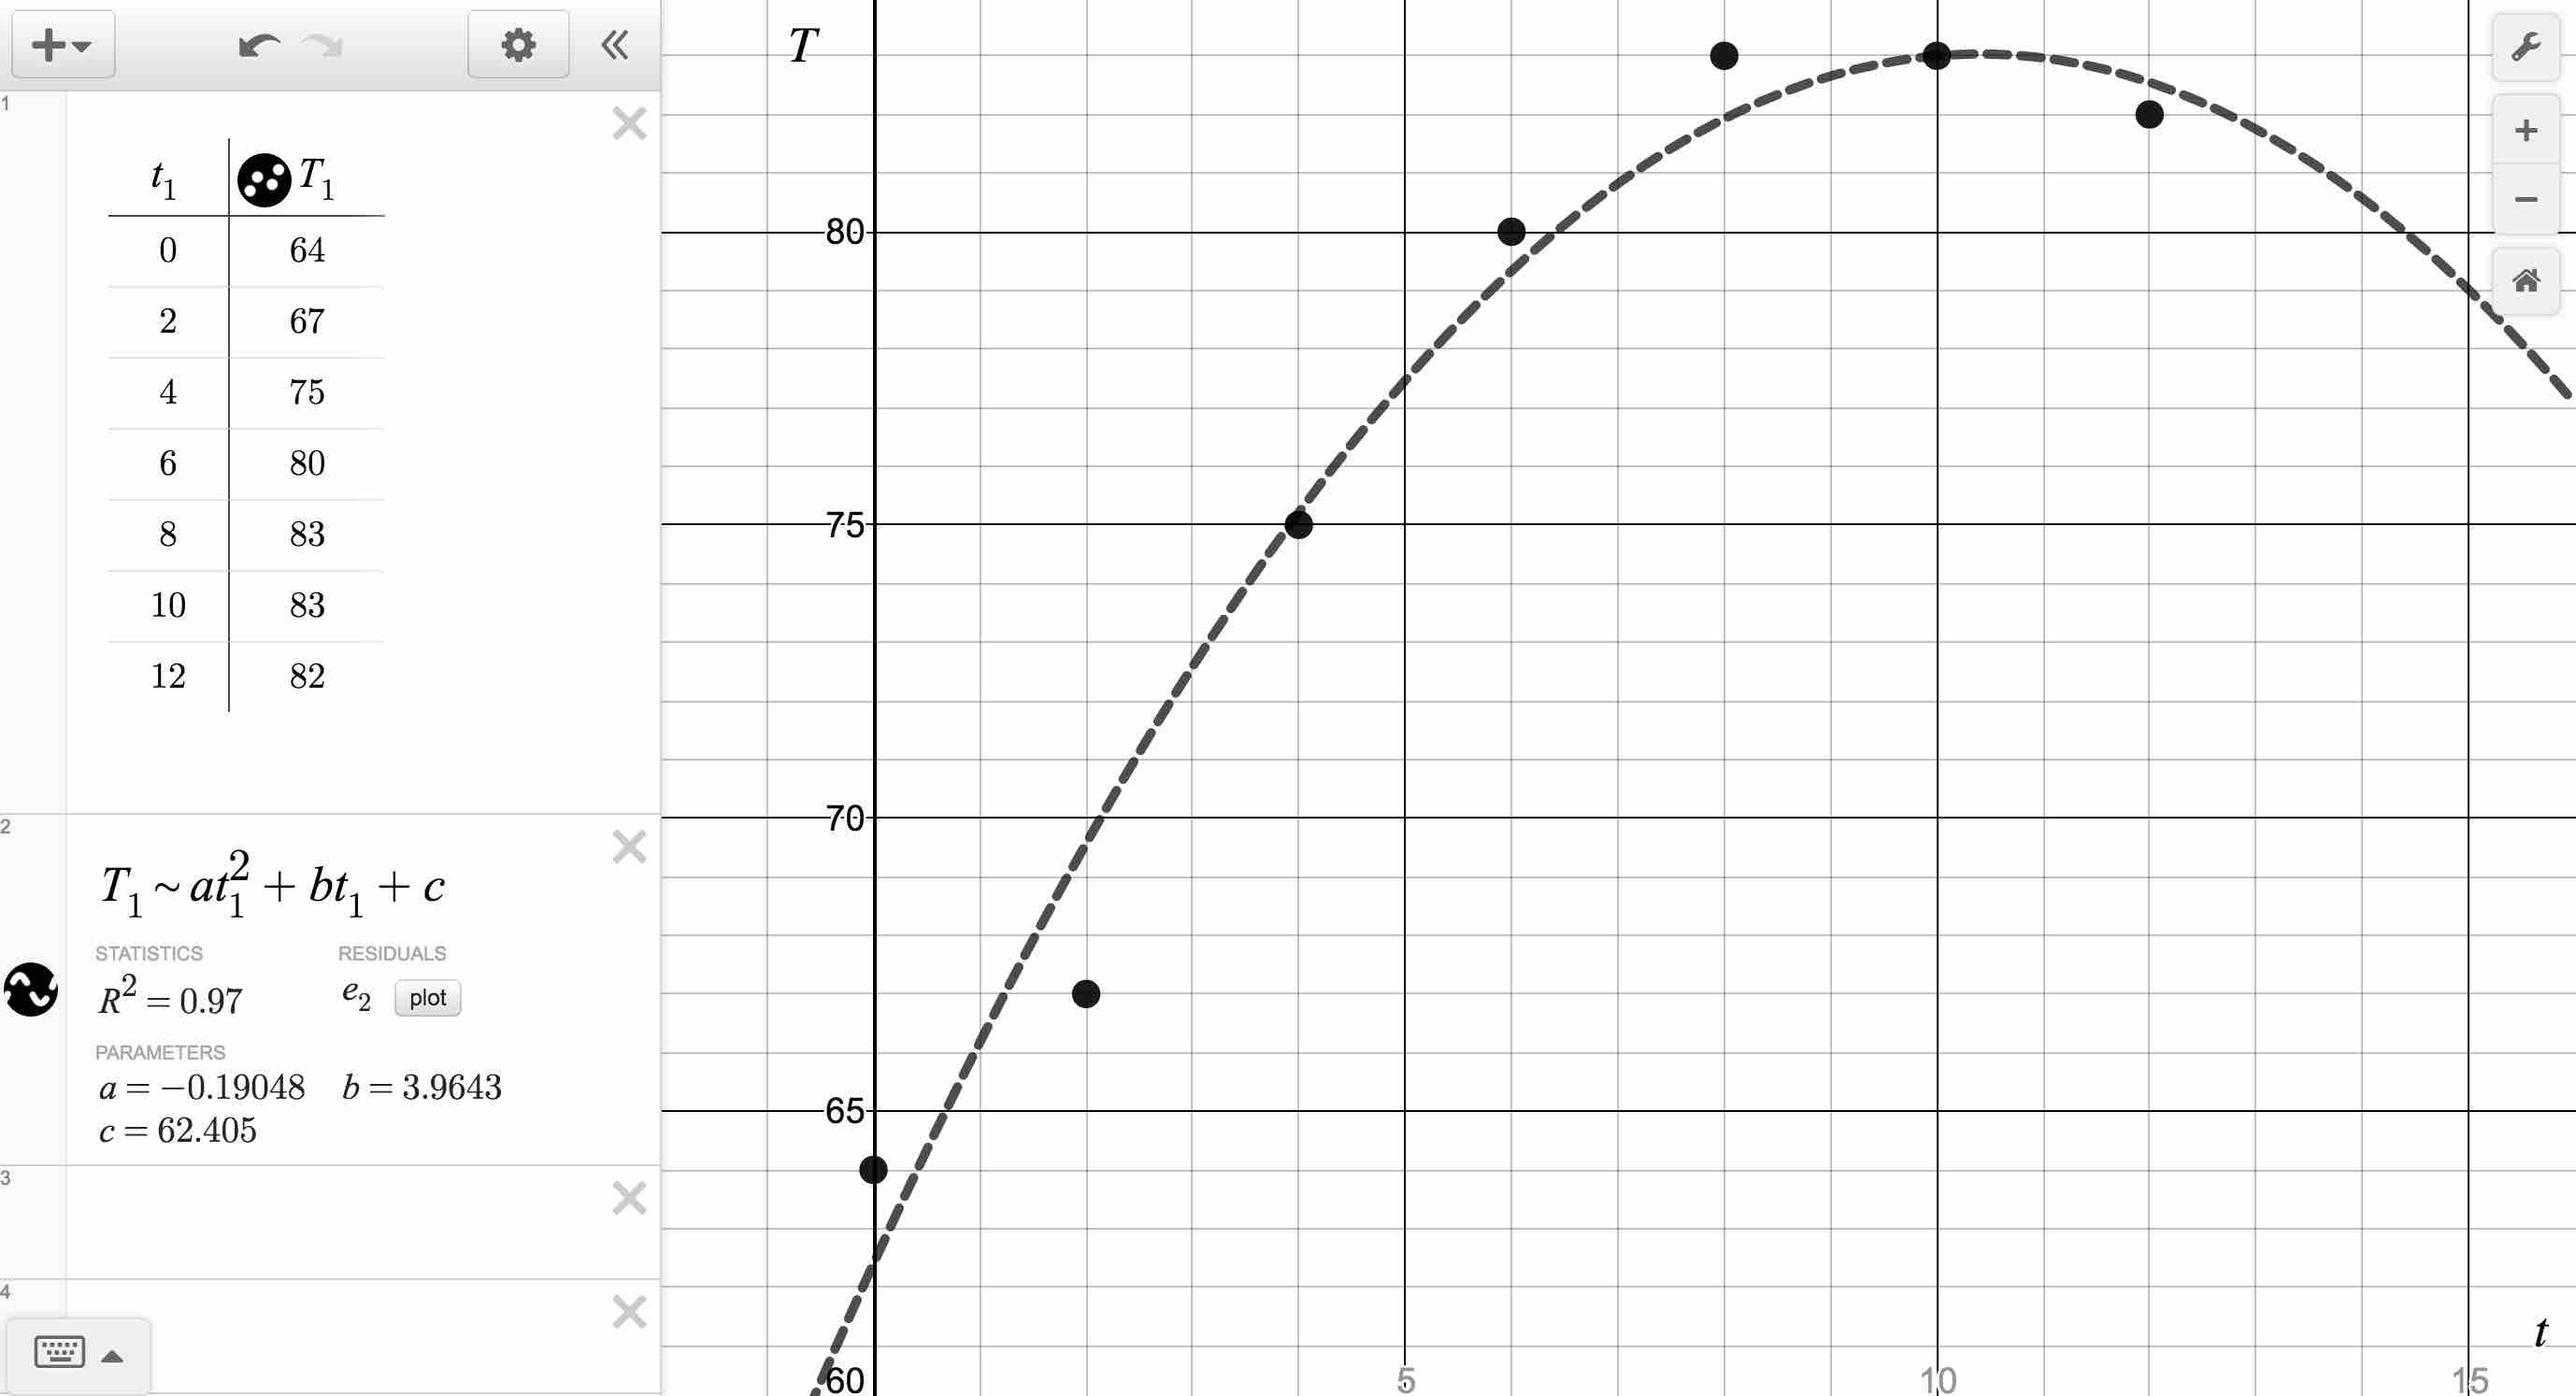
\includegraphics[width=5in]{./QuadraticFunctionsGraphics/TimeTempDataQR.jpg}
 
 \end{center}
 
 \qed
 
 \end{enumerate}
 
 \end{ex}

It is interesting how close the predictions from  Examples \ref{timetempregressionex} and  \ref{TimeTempQRex} despite one using linear models and one using a quadratic model.  Which model is the `better' model?  We leave that discussion to the reader and their classmates.

\medskip
}

Our next example is classic application of optimizing a quadratic function.

\begin{ex} \label{donniealpaca} Much to Donnie's surprise and delight, he inherits a large parcel of land in Ashtabula County from one of his (e)strange(d) relatives so the time is right for him to pursue his dream of raising alpaca.  He wishes to build a rectangular pasture and estimates that he has enough money for 200 linear feet of fencing material.  If he makes the pasture adjacent to a river (so that no fencing is required on that side), what are the dimensions of the pasture which maximize the area?  What is the maximum area?  If an average alpaca needs 25 square feet of grazing area, how many alpaca can Donnie keep in his pasture?

%\pagebreak

{\bf Solution.} We are asked to find the dimensions of the pasture which would give a maximum area, so we begin by sketching the diagram seen below on the left.  We let $w$ denote the width of the pasture and we let $\ell$ denote the length of the pasture.  The units given to us in the statement of the problem are feet, so we assume that $w$ and $\ell$ are measured in feet.  The area of the pasture, which we'll call $A$, is related to $w$ and $\ell$ by the equation $A = w \ell$.  Since $w$ and $\ell$ are both measured in feet, $A$ has units of $\text{feet}^2$, or square feet.  

\medskip

We are also told that the total amount of fencing available is $200$ feet, which means $w + \ell + w = 200$, or, $\ell+2w = 200$.  We now have two equations, $A = w \ell$ and $\ell+2w = 200$.  In order to use the tools given to us in this section to \textit{maximize} $A$, we need to use the information given to write $A$ as a function of just \textit{one} variable, either $w$ or $\ell$. This is where we use the equation $\ell+2w = 200$.  Solving for $\ell$, we find $\ell = 200-2w$, and we substitute this into our equation for $A$.  We get $A = w \ell = w(200-2w) = 200w-2w^2$.  We now have $A$ as a function of $w$, $A = f(w) = 200w-2w^2 = -2w^2+200w$. 

\begin{center}

\setlength\columnsep{0pt}

\begin{multicols}{2}

\begin{mfpic}[15]{-4}{4}{0}{4}
\fillcolor[gray]{0.8}
\gfill \rect{(-4,2), (4,4)}

\dashed \polyline{(-3,2), (-3,0.5), (3,0.5), (3,2)}
\tlabel[cc](-3.5,1.25){$w$}
\tlabel[cc](0,0){$\ell$}
\tlabel[cc](3.5, 1.25){$w$}
\tlabel[cc](0,1.25){pasture}
\tlabel[cc](0,3){river} 

\penwd{1.25pt}
\polyline{(-4,2), (4,2)}
\polyline{(-4,4), (4,4)}


\end{mfpic}

\begin{mfpic}[15]{-1}{10.75}{-1}{6}
\axes
\tlabel[cc](11,0){\scriptsize  $w$}
\tlabel[cc](0.5,6){\scriptsize  $A$}
\tlabel[cc](5,5.5){\scriptsize  $(50, 5000)$}
\tlabel[cc](-0.75,-0.5){\scriptsize  $(0, 0)$}
\tlabel[cc](10,-0.5){\scriptsize $(100, 0)$}
\tlabel[cc](5,5.5){\scriptsize  $(50, 5000)$}
\tcaption{\scriptsize $A = f(w)$}
\xmarks{1 step 1 until 10}
\ymarks{1 step 1 until 5}
\scriptsize
\tlpointsep{4pt}
\axislabels {x}{ {$10$} 1, {$30$} 3,  {$50$} 5,{$70$} 7}
\axislabels {y}{{$1000$} 1, {$2000$} 2, {$3000$} 3, {$4000$} 4, {$5000$} 5}
\normalsize
\penwd{1.25pt}
\function{0,10,0.1}{(0-0.2)*(x**2) + 2*x}
\point[4pt]{(5,5)}
\pointfillfalse
\point[4pt]{(0,0), (10,0)}

\end{mfpic}

\end{multicols}

\setlength\columnsep{10pt}

\end{center}

Before we go any further, we need to find the applied domain of $f$ so that we know what values of $w$ make sense in this situation.\footnote{Donnie would be very upset if, for example, we told him the width of the pasture needs to be $-50$ feet.}  Given that $w$ represents the width of the pasture we need $w > 0$.  Likewise, $\ell$ represents the length of the pasture, so $\ell = 200-2w > 0$.  Solving this latter inequality yields $w < 100$.  Hence, the function we wish to maximize is $f(w) = -2w^2 + 200w$ for $0 < w < 100$.  We know two things about the quadratic function $f$: the graph of $A = f(w)$ is a parabola and (since the coefficient of $w^2$ is $-2$) the parabola opens downwards.  

\medskip

This means that there is a maximum value to be found, and we know it occurs at the vertex.  Using the vertex formula, we find $w = -\frac{200}{2(-2)} = 50$, and $A = f(50) = -2(50)^2 + 200(50) = 5000$.  Since $w=50$ lies in the applied domain, $0 < w < 100$, we have that the area of the pasture is maximized when the width is $50$ feet.  To find the length, we use $\ell = 200-2w$ and find $ \ell = 200-2(50) = 100$, so the length of the pasture is $100$ feet.  The maximum area is $A =f(50) = 5000$, or $5000$ square feet.  If an average alpaca requires 25 square feet of pasture, Donnie can raise $\frac{5000}{25} = 200$ average alpaca. \qed

\end{ex}

The function $f$ in Example \ref{donniealpaca} is called the\index{objective function}\index{optimization ! objective function} \textbf{objective function} for this problem - it's the function we're trying to optimize.  In the case above, we were trying to maximize $f$. The equation  $\ell+2w = 200$ along with the inequalities $w>0$ and $\ell >0$ are called the\index{constraint}\index{optimization ! constraint} \textbf{constraints}.   As we saw in this example, and as we'll see again and again, the constraint equation is used to rewrite the objective function in terms of just one of the variables where constraint inequalities, if any, help determine the applied domain.

\begin{comment}
\subsection{Inequalities involving Quadratic Functions}
\label{QuadraticInequalities}


We now turn our attention to solving inequalities involving quadratic functions.   Consider the inequality $x^2 \leq 6$.  We could use the fact that the square root is increasing\footnote{That is, if $a < b$, then $\sqrt{a} < \sqrt{b}$.} to get: $\sqrt{x^2} \leq \sqrt{6}$, or $|x| \leq \sqrt{6}$.  This reduces to $-\sqrt{6} \leq x \leq \sqrt{6}$ or, using interval notation, $[-\sqrt{6}, \sqrt{6}]$. If, however, we had to solve $x^2 \leq x+6$, things are more complicated.  One approach is to complete the square: \[ \begin{array}{rcl}

x^2 & \leq & x+6 \\
x^2 - x & \leq & 6 \\
x^2 - x + \frac{1}{4} & \leq &  6 + \frac{1}{4} \\ [3pt]

\left(x - \frac{1}{2} \right)^2 & \leq & \frac{25}{4} \\ [3pt]

\sqrt{\left(x - \frac{1}{2} \right)^2} & \leq & \sqrt{\frac{25}{4}} \\ [3pt]

\left| x - \frac{1}{2} \right| & \leq & \frac{5}{2} \\ 

-\frac{5}{2} \quad \leq & x - \frac{1}{2} & \leq \quad \frac{5}{2} \\ 

-2 \quad &  \leq  x  \leq & 3 \\  \end{array} \] We get the solution $[-2,3]$.  While there is nothing wrong with this approach, we seek methods here that will generalize to higher degree polynomials such as those we'll see in Chapter \ref{PolynomialFunctions}.  

\medskip

To that end, we look at the inequality $x^2 \leq x+6$ graphically.  Identifying $f(x) = x^2$ and $g(x) = x+6$ , we graph $f$ and $g$ on the same set of axes below on the left and look for where the graph of $f$ (the parabola) meets or is below the graph of $g$ (the line).  There are two points of intersection which we determine by solving  $f(x) = g(x)$ or $x^2=x+6$.  As usual, we rewrite this equation as $x^2-x-6 = 0$ in order to use the primary tools we've developed to handle these types\footnote{Namely ones with a nonzero coefficient of `$x$'.} of quadratic equations: factoring, or failing that, the Quadratic Formula.  We find $x^2-x-6 = (x+2)(x-3)$ so we get two solutions to $(x+2)(x-3) = 0$, namely $x = -2$ and $x = 3$.  Putting these together with the graph, we obtain the same solution:  $[-2,3]$.  

\begin{center}

\begin{multicols}{2}

\begin{mfpic}[15]{-4}{4}{-1}{10}
\axes
\tlabel[cc](4,-0.5){\scriptsize $x$}
\tlabel[cc](0.5,10){\scriptsize $y$}
\xmarks{-3 step 1 until 3}
\ymarks{1 step 1 until 9}
\scriptsize
\tlabel[cc](-3,4){\scriptsize $(-2,4)$}
\tlabel[cc](4,9){\scriptsize $(3,9)$}
\tlpointsep{4pt}
\axislabels {x}{{$-3 \hspace{7pt}$} -3, {$-2 \hspace{7pt}$} -2, {$-1 \hspace{7pt}$} -1, {$1$} 1, {$2$} 2, {$3$} 3}
\axislabels {y}{{$1$} 1, {$2$} 2, {$3$} 3, {$4$} 4, {$5$} 5, {$6$} 6, {$7$} 7, {$8$} 8, {$9$} 9}
\tcaption{\scriptsize Solving $x^2 \leq x+6$.}
\normalsize
\arrow \reverse \arrow \function{-3.15,3.15,0.1}{x**2}
\arrow \reverse \arrow \polyline{(-4,2), (4,10)}
\penwd{1.25pt}
\function{-2,3,0.1}{x**2}
\polyline{(-2,4), (3,9)}
\point[4pt]{(-2,0),(3,0), (-2,4), (3,9)}
\polyline{(-2,0), (3,0)}
\end{mfpic}


\begin{mfpic}[11.78]{-4}{4}{-7}{7}
\axes
\tlabel[cc](4,-0.5){\scriptsize $x$}
\tlabel[cc](0.5,7){\scriptsize $y$}
\tlabel[cc](-3.5,0.5){\scriptsize $(-2,0)$}
\tlabel[cc](2,0.5){\scriptsize $(3,0)$}
\xmarks{-3 step 1 until 3}
\ymarks{-5 step 1 until 6}
\scriptsize
\tlpointsep{4pt}
\axislabels {x}{{$-3 \hspace{7pt}$} -3,  {$-1 \hspace{7pt}$} -1, {$1$} 1, {$2$} 2}
\axislabels {y}{{$-6$} -6,  {$-4$} -4,{$-2$} -2,   {$2$} 2, {$4$} 4,  {$6$} 6}
\tcaption{\scriptsize Solving $x^2-x-6 \leq 0$.}
\normalsize
\arrow \reverse \arrow \function{-3,4,0.1}{x**2-x-6}
\penwd{1.25pt}
\function{-2,3,0.1}{x**2-x-6}
\polyline{(-2,0), (3,0)}
\point[4pt]{(-2,0),(3,0)}
\end{mfpic}

\end{multicols}

\end{center}

Yet a third way to attack $x^2 \leq x+6$ is to rewrite the inequality as $x^2-x-6 \leq 0$.  Here, we graph $f(x) = x^2-x-6$ to look for where the graph meets or is below the graph of $g(x) = 0$, a.k.a. the $x$-axis.  Doing so requires us to find the zeros of $f$, that is, solve $f(x) = x^2-x-6=0$ from which we obtain $x =-2$ and $x = 3$ as before.  We find the same solution, $[-2,3]$ as is showcased in the graph at the bottom of the previous page on the right.  

\medskip

One advantage to using this last approach is that we are essentially concerned with \text{one} function and its \textit{zeros}.  This approach can be generalized to all functions - not just quadratics, so we take the time to develop this method more thoroughly now.  

\phantomsection
\label{firstsigndiagram}

\medskip

Consider the graph of $f(x) = x^2-x-6$ below  The zeros of $f$ are $x=-2$ and $x=3$ and they divide the domain (the $x$-axis) into three intervals:  $(-\infty, -2)$, $(-2,3)$ and $(3, \infty)$.  For every number in $(-\infty, -2)$, the graph of $f$ is above the $x$-axis; in other words, $f(x) > 0$ for all $x$ in $(-\infty, -2)$. Similarly, $f(x) < 0$ for all $x$ in $(-2,3)$, and $f(x) > 0$ for all $x$ in $(3, \infty)$.  We represent this schematically with the {\bf sign diagram} below.\index{inequality ! sign diagram}\index{sign diagram ! for quadratic inequality} 

\begin{center}

\begin{multicols}{2}

\begin{mfpic}[12]{-4}{4}{-7}{7}
\axes
\tlabel[cc](4,-0.5){\scriptsize $x$}
\tlabel[cc](0.5,7){\scriptsize $y$}
\tlabel[cc](-3.5,0.5){\scriptsize $(-2,0)$}
\tlabel[cc](2,0.5){\scriptsize $(3,0)$}
\xmarks{-3 step 1 until 3}
\ymarks{-5 step 1 until 6}
\scriptsize
\tlpointsep{4pt}
\axislabels {x}{{$-3 \hspace{7pt}$} -3,  {$-1 \hspace{7pt}$} -1, {$1$} 1, {$2$} 2}
\axislabels {y}{{$-6$} -6,  {$-4$} -4,{$-2$} -2,   {$2$} 2, {$4$} 4,  {$6$} 6}
\tcaption{ $f(x) = x^2-x-6$.}
\normalsize
\penwd{1.25pt}
\arrow \reverse \arrow \function{-3,4,0.1}{x**2-x-6}
\point[4pt]{(-2,0),(3,0)}
\end{mfpic} 

\columnbreak

\vspace*{0.75in}
\begin{mfpic}[15]{-5}{5}{-5}{6}
\arrow \reverse \arrow \polyline{(-5,0),(5,0)}
\xmarks{-2,2}
\tcaption{A sign diagram for $f(x) = x^2-x-6$}
\tlpointsep{4pt}
\axislabels {x}{{$-2 \hspace{7pt}$} -2, {$3$} 2}
\tlabel[cc](-3.5,1){$(+)$}
\tlabel[cc](-2,1){$0$}
\tlabel[cc](0,1){$(-)$}
\tlabel[cc](2,1){$0$}
\tlabel[cc](3.5,1){$(+)$}
\end{mfpic}

\end{multicols}

\end{center}

The $(+)$ above a portion of the number line indicates $f(x) > 0$ for those values of $x$ and the $(-)$ indicates $f(x) < 0$ there.  The numbers labeled on the number line are the zeros of $f$, so we place $0$ above them.  For the inequality $f(x) = x^2-x-6 \leq 0$, we read from the sign diagram that the solution is $[-2,3]$.  

\medskip

Our next goal is to establish a procedure by which we can generate the sign diagram without graphing the function.  While parabolas aren't that bad to graph knowing what we know, our sights are set on more general functions whose graphs are more complicated.  

\medskip
\enlargethispage{.in}

An important property of parabolas is that a parabola can't be above the $x$-axis at one point and below the $x$-axis at another point without crossing the $x$-axis at some point in between. Said differently, if the function is positive at one point and negative at another, the function must have at least one zero in between.  This property is a consequence of quadratic functions being\index{function ! continuous}\index{continuous} \textbf{continuous}.  A precise definition of `continuous' requires the language of Calculus, but it suffices for us to know that the graph of a continuous function has no gaps or holes.   This allows us to determine the sign of \emph{all} of the function values on a given interval by testing the function at just \emph{one} value in the interval.  

\medskip

The result below applies to all continuous functions defined on an interval of real numbers, but we restrict our attention to quadratic functions for the time being,

\medskip

\colorbox{ResultColor}{\bbm

\centerline{\textbf{Steps for Creating A Sign Diagram for A Quadratic Function}} \index{sign diagram ! creating }

\smallskip

Suppose $f$ is a quadratic function.

\begin{enumerate}

\item  Find the zeros of $f$ and place them on the number line with the number $0$ above them.

\item  Choose a real number, called a \textbf{test value}, in each of the intervals determined in step 1. 

\item  Determine and record the sign of $f(x)$ for each test value in step 2.

\end{enumerate}

\ebm}

\medskip

To use a sign diagram to solve an inequality, we must always remember to compare the function to $0$.

\medskip

\colorbox{ResultColor}{\bbm

\centerline{\textbf{Solving Inequalities using Sign Diagrams}} \index{inequality ! solution using sign diagram }

\smallskip

To solve an inequality using a sign diagram:

\begin{enumerate}

\item  Rewrite the inequality so some function $f(x)$ is being compared to `$0$.'

\item  Make a sign diagram for $f$.

\item  Record the solution.

\end{enumerate}

\ebm}

\medskip

We practice this approach in the following example.

\begin{ex}  Solve the following inequalities analytically\footnote{By `solve analytically' we mean `algebraically' using a sign diagram.} and check your solutions graphically.

\begin{multicols}{2}
\begin{enumerate}

\item  $2x^2 \leq 3-x$

\item  $t^2 - 2t > 1$

\setcounter{HW}{\value{enumi}}
\end{enumerate}
\end{multicols}

\begin{multicols}{2}
\begin{enumerate}
\setcounter{enumi}{\value{HW}}

\item  $x^2+1 \leq 2x$

\item  $2t-t^2 \geq |t-1|-1$

\end{enumerate}
\end{multicols}

{\bf Solution.}  

\begin{enumerate}

\item  To solve $2x^2 \leq 3-x$, we rewrite it as $2x^2+x-3 \leq 0$.  We find the zeros of $f(x) = 2x^2 + x - 3$ by solving $2x^2 + x - 3 = 0$.  Factoring gives $(2x+3)(x-1)=0$, so $x = -\frac{3}{2}$ or $x = 1$.  We place these values on the number line with $0$ above them and choose test values in the intervals $\left(-\infty, -\frac{3}{2}\right)$, $\left(-\frac{3}{2},1\right)$ and $(1,\infty)$.  For the interval  $\left(-\infty, -\frac{3}{2}\right)$, we choose\footnote{We have to choose \textit{something} in each interval.  If you don't like our choices, please feel free to choose different numbers.  You'll get the same sign chart.} $x=-2$; for $\left(-\frac{3}{2},1\right)$, we pick $x=0$; and for $(1,\infty)$, $x=2$. Evaluating the function at the three test values gives us $f(-2) = 3 > 0$, so we place $(+)$ above $\left(-\infty, -\frac{3}{2}\right)$;  $f(0)=-3 < 0$, so $(-)$ goes above the interval $\left(-\frac{3}{2},1\right)$;  and, $f(2) = 7$, which means $(+)$ is placed above $(1,\infty)$.

\medskip

We are solving $2x^2+x-3 \leq 0$ so we need solutions to $2x^2+x-3 < 0$ as well as solutions for $2x^2+x-3 =0$.  For $2x^2+x-3 < 0$, we need the intervals which we have a $(-)$ above them.  The sign diagram shows only one: $\left(-\frac{3}{2},1\right)$.  Also, we know $2x^2+x-3 =0$ when $x=-\frac{3}{2}$ and $x=1$, so our final answer is $\left[-\frac{3}{2},1\right]$.  

\medskip

To verify our solution graphically, we refer to the original inequality, $2x^2 \leq 3-x$.  We let $g(x) = 2x^2$ and $h(x)=3-x$.  We are looking for the $x$ values where the graph of $g$ is below that of $h$ (the solution to $g(x) < h(x)$) as well as the points of intersection (the solutions to $g(x)=h(x)$).  The graphs of $g$ and $h$ are given on the right with the sign chart on the left.


\begin{center}

\begin{multicols}{2}

\vspace*{.25in}

\begin{mfpic}[15]{-5}{5}{-2}{2}
\arrow \reverse \arrow \polyline{(-5,0),(5,0)}
\xmarks{-2,2}
\arrow \polyline{(-3.5,-1.5),(-3.5,-0.5)}
\arrow \polyline{(0,-1.5),(0,-0.5)}
\arrow \polyline{(3.5,-1.5),(3.5,-0.5)}
\tlpointsep{4pt}
%\scriptsize
\axislabels {x}{{$-\frac{3}{2} \hspace{7pt}$} -2, {$1$} 2}
\tlabel[cc](-3.5,1){$(+)$}
\tlabel[cc](-2,1){$0$}
\tlabel[cc](0,1){$(-)$}
\tlabel[cc](2,1){$0$}
\tlabel[cc](3.5,1){$(+)$}
\tlabel[cc](-3.75,-2.25){$-2$}
\tlabel[cc](-0.1,-2.25){$0$}
\tlabel[cc](3.4,-2.25){$2$}
%\normalsize
\end{mfpic}  

\columnbreak

\begin{mfpic}[20][10]{-3}{3}{-1}{8}
\arrow \reverse \arrow \function{-2,2,0.1}{2*(x**2)}
\arrow \reverse \arrow \polyline{(-3,6),(2.5,0.5)}
\xmarks{-2 step 1 until 2}
\ymarks{1 step 1 until 7}
\axes
\tlabel[cc](3,-0.5){\scriptsize $x$}
\tlabel[cc](0.5,8){\scriptsize $y$}
\tlabel[cc](2.75,6){\scriptsize $y=2x^2$}
\tlabel[cc](3,1.75){\scriptsize $y=3-x$}
\scriptsize
\tlpointsep{4pt}
\axislabels {x}{{$-2 \hspace{7pt}$} -2, {$-1 \hspace{7pt}$} -1,{$1$} 1, {$2$} 2}
\axislabels {y}{{$2$} 2, {$3$} 3, {$4$} 4, {$5$} 5, {$6$} 6, {$7$} 7}
\normalsize 
\penwd{1.25pt} 
 \function{-1.5,1,0.1}{2*(x**2)}
 \polyline{(-1.5,4.5),(1,2)}
\polyline{(-1.5,0), (1,0)}
\point[4pt]{(-1.5,0), (1,0), (-1.5, 4.5), (1,2)}
\end{mfpic}

\end{multicols}

\end{center}

\item Once again, we re-write  $t^2-2t > 1$ as $t^2-2t-1>0$ and we identify $f(t)=t^2-2t-1$.  When we go to find the zeros of $f$, we find, to our chagrin, that the quadratic $t^2-2t-1$ doesn't factor nicely.  Hence, we resort to  the Quadratic Formula and find $t=1 \pm \sqrt{2}$.  As before, these zeros divide the number line into three pieces.  To help us decide on test values, we approximate $1 - \sqrt{2} \approx -0.4$ and $1 + \sqrt{2} \approx 2.4$.  We choose $t=-1$, $t=0$ and $t=3$ as our test values and find $f(-1)= 2$, which is $(+)$; $f(0)=-1$ which is $(-)$; and $f(3)=2$ which is $(+)$ again.  Our solution to $t^2-2t-1>0$ is where we have $(+)$, so, in interval notation $\left(-\infty, 1-\sqrt{2}\right) \cup \left(1+\sqrt{2},\infty\right)$.  

\medskip

To check the inequality $t^2 - 2t > 1$ graphically, we set $g(t) = t^2-2t$ and $h(t)=1$.  We are looking for the $t$ values where the graph of $g$ is above the graph of $h$.  As before we present the graphs on the right and the sign chart on the left.

\begin{center}

\begin{multicols}{2}

\vspace*{.25in}

\begin{mfpic}[14]{-8}{8}{-2}{2}
\arrow \reverse \arrow \polyline{(-8,0),(8,0)}
\xmarks{-3,3}
\arrow \polyline{(-6,-1.5),(-6,-0.5)}
\arrow \polyline{(0,-1.5),(0,-0.5)}
\arrow \polyline{(6,-1.5),(6,-0.5)}
\tlpointsep{4pt}
%\scriptsize
\axislabels {x}{{$1-\sqrt{2}$} -3, {$1+\sqrt{2}$} 3}
\tlabel[cc](-6,1){$(+)$}
\tlabel[cc](-3,1){$0$}
\tlabel[cc](0,1){$(-)$}
\tlabel[cc](3,1){$0$}
\tlabel[cc](6,1){$(+)$}
\tlabel[cc](-6,-2.25){$-1$}
\tlabel[cc](0,-2.25){$0$}
\tlabel[cc](6,-2.25){$3$}
%\normalsize
\end{mfpic} 

\columnbreak

\begin{mfpic}[20]{-4}{4}{-1}{4}
\arrow \reverse \arrow \function{-1.23,3.21,0.1}{(x**2)-2*x}
\arrow \reverse \arrow \function{-4,4,0.1}{1}
\xmarks{-3 step 1 until 3}
\ymarks{1 step 1 until 3}
\axes
\tlabel[cc](4,-0.5){\scriptsize $t$}
\tlabel[cc](0.5,4){\scriptsize $y$}
\tlabel[cc](-2.5,1.25){\scriptsize $y=1$}
\tlabel[cc](2.75,-1){\scriptsize $y=t^2-2t$}
\scriptsize
\tlpointsep{4pt}
\axislabels {x}{{$-3 \hspace{7pt}$} -3,{$-2 \hspace{7pt}$} -2,{$-1 \hspace{7pt}$} -1,{$1$} 1, {$2$} 2, {$3$} 3}
\axislabels {y}{{$2$} 2, {$3$} 3}
\normalsize 
\penwd{1.25pt} 
\arrow \reverse \function{-1.23,-0.4142,0.1}{(x**2)-2*x}
\arrow \function{2.4142,3.21,0.1}{(x**2)-2*x}
\arrow \polyline{(-0.4142,0), (-4,0)}
\arrow \polyline{(2.4142,0), (4,0)}
\arrow \polyline{(-0.4142,1), (-4,1)}
\arrow \polyline{(2.4142,1), (4,1)}
\pointfillfalse
\point[4pt]{(-0.4142,0),(2.4142,0)}
\point[4pt]{(-0.4142,1),(2.4142,1)}
\end{mfpic}

\end{multicols}

\end{center}


\item  To solve  $x^2+1 \leq 2x$, as before, we solve  $x^2-2x+1 \leq 0$.  Setting $f(x) = x^2-2x+1=0$, we find only one zero of $f$: $x = 1$.  This one $x$ value divides the number line into two intervals, from which we choose $x=0$ and $x=2$ as test values.  We find $f(0)=1 > 0$ and $f(2) = 1 > 0$.  Since we are looking for solutions to $x^2-2x+1 \leq 0$, we are looking for $x$ values where $x^2-2x+1 < 0$ as well as where $x^2-2x+1 = 0$.  Looking at our sign diagram, there are no places where $x^2-2x+1 < 0$ (there are no $(-)$), so our solution is only $x=1$ (where $x^2-2x+1 = 0$).  We write this as $\left\{1\right\}$.  

\medskip

Graphically, we solve $x^2+1 \leq 2x$ by graphing $g(x) = x^2+1$ and $h(x)=2x$. We are looking for the $x$ values where the graph of $g$ is below the graph of $h$ (for $x^2+1 < 2x$) and where the two graphs intersect ($x^2+1 = 2x$).  Notice that the line and the parabola touch at $\left(1, 2\right)$, but the parabola is always above the line otherwise.\footnote{In this case, we say the line $y=2x$ is \textbf{tangent} to $y=x^2+1$ at $\left(1, 2\right)$.  Finding tangent lines to arbitrary functions is a fundamental problem solved, in general, with Calculus.}

\begin{center}

\begin{multicols}{2}

\vspace*{.25in}

\begin{mfpic}[15]{-5}{5}{-2}{2}
\arrow \reverse \arrow \polyline{(-5,0),(5,0)}
\xmarks{0}
\arrow \polyline{(-2.5,-1.5),(-2.5,-0.5)}
\arrow \polyline{(2.5,-1.5),(2.5,-0.5)}
\tlpointsep{4pt}
%\scriptsize
\axislabels {x}{{$1$} 0}
\tlabel[cc](-2.5,1){$(+)$}
\tlabel[cc](0,1){$0$}
\tlabel[cc](2.5,1){$(+)$}
\tlabel[cc](-2.6,-2.1){$0$}
\tlabel[cc](2.4,-2.1){$2$}
%\normalsize
\end{mfpic}  

\columnbreak

\begin{mfpic}[20]{-2}{2}{-1}{5}
\arrow \reverse \arrow \function{-2,2,0.1}{(x**2)+1}
\arrow \reverse \arrow \function{-0.5,2.5,0.1}{2*x}
\point[4pt]{(1,2), (1,0)}
\xmarks{-1 step 1 until 1}
\ymarks{1 step 1 until 4}
\axes
\tlabel[cc](2,-0.5){\scriptsize $x$}
\tlabel[cc](0.5,5){\scriptsize $y$}
\tlabel[cc](1,0.5){\scriptsize $y=2x$}
\tlabel[cc](-2.25,2){\scriptsize $y=x^2+1$}
\scriptsize
\tlpointsep{4pt}
\axislabels {x}{{$-1 \hspace{7pt}$} -1,{$1$} 1}
\axislabels {y}{{$1$} 1,{$2$} 2, {$3$} 3, {$4$} 4}
\normalsize 
\end{mfpic}

\end{multicols}

\end{center}

\item  To solve $2t-t^2 \geq |t-1|-1$ analytically we first rewrite the absolute value using cases.  For $t< 1$, $|t-1| = -(t-1) = -t+1$, so we get $2t-t^2 \geq (-t+1)-1$ which simplifies to  $t^2-3t \leq 0$.  Finding the zeros of $f(t) = t^2-3t$, we get $t=0$ and $t=3$.  However, we are concerned only with the portion of the number line where $t < 1$, so the only zero that we deal with is $t=0$.  This divides the interval $t<1$ into two intervals:  $(-\infty, 0)$ and $(0,1)$.  We choose $t=-1$ and $t=\frac{1}{2}$ as our test values.  We find $f(-1) = 4$ and $f\left(\frac{1}{2}\right) = -\frac{5}{4}$.  Hence, our solution to $t^2-3t \leq 0$ for $t < 1$ is $[0,1)$. 

 Next, we turn our attention to the case $t \geq 1$.  Here, $|t-1| = t-1$, so our original inequality becomes $2t-t^2 \geq (t-1)-1$, or $t^2-t-2 \leq 0$.  Setting $g(t) = t^2-t-2$, we find the zeros of $g$ to be $t=-1$ and $t=2$.  Of these, only $t=2$ lies in the region $t\geq 1$, so we ignore $t=-1$.  Our test intervals are now $[1,2)$ and $(2,\infty)$.  We choose $t=1$ and $t=3$ as our test values and find $g(1) = -2$ and $g(3) = 4$.  Hence, our solution to $g(t) = t^2-t-2 \leq 0$, in this region is $[1,2)$.

\begin{center}

\begin{multicols}{2}

\begin{mfpic}[15]{-5}{5.5}{-2}{2}
\arrow \reverse \polyline{(-5,0),(5,0)}
\xmarks{0}
\arrow \polyline{(-2.5,-1.5),(-2.5,-0.5)}
\arrow \polyline{(2.5,-1.25),(2.5,-0.5)}
\tlpointsep{4pt}
%\scriptsize
\axislabels {x}{{$0$} 0}
\tlabel[cc](-2.5,1){$(+)$}
\tlabel[cc](0,1){$0$}
\tlabel[cc](2.5,1){$(-)$}
\tlabel[cc](-2.5,-2.25){$-1$}
\tlabel[cc](2.5,-2.25){$\frac{1}{2}$}
\gclear \circle{(5,0),0.2}
\circle{(5,0),0.2}
\tlabel[cc](5,-0.75){$1$}
%\normalsize
\end{mfpic}  

Solving $2t-t^2 \geq |t-1|-1$ for $t < 1$. 

\columnbreak

\begin{mfpic}[15]{-5}{5.5}{-2}{2}
\arrow \polyline{(-5,0),(5,0)}
\xmarks{0}
\arrow \polyline{(-5,-1.5),(-5,-0.5)}
\arrow \polyline{(2.5,-1.5),(2.5,-0.5)}
\tlpointsep{4pt}
%\scriptsize
\axislabels {x}{{$2$} 0}
\tlabel[cc](-2.5,1){$(-)$}
\tlabel[cc](0,1){$0$}
\tlabel[cc](2.5,1){$(+)$}
\tlabel[cc](2.5,-2.25){$3$}
\gfill \circle{(-5,0),0.2}
\tlabel[cc](-5,-2.25){$1$}
%\normalsize
\end{mfpic} 

Solving $2t-t^2 \geq |t-1|-1$ for $t \geq 1$.  

\end{multicols}

\end{center}

Combining these into one sign diagram, we have that our solution is $[0,2]$.  Graphically, to check $2t-t^2 \geq |t-1|-1$, we set $h(t) = 2t-t^2$ and $i(t) = |t-1|-1$ and look for the $t$ values where the graph of $h$ intersects or is above the the graph of $i$ The combined sign chart is given on the left and the graphs are on the right.

\begin{center}

\begin{multicols}{2} \raggedcolumns

\vspace*{.35in}

\begin{mfpic}[15]{-5}{5}{-2}{2}
\arrow \reverse \arrow \polyline{(-5,0),(5,0)}
\xmarks{-2,2}
\arrow \polyline{(-3.5,-1.5),(-3.5,-0.5)}
\arrow \polyline{(0,-1.5),(0,-0.5)}
\arrow \polyline{(3.75,-1.5),(3.75,-0.5)}
\tlpointsep{4pt}
%\scriptsize
\axislabels {x}{{$0$} -2, {$2$} 2}
\tlabel[cc](-3.5,1){$(+)$}
\tlabel[cc](-2,1){$0$}
\tlabel[cc](0,1){$(-)$}
\tlabel[cc](2,1){$0$}
\tlabel[cc](3.5,1){$(+)$}
\tlabel[cc](-3.55,-2.25){$-1$}
\tlabel[cc](-0.05,-2.25){$0$}
\tlabel[cc](3.7,-2.25){$3$}
%\normalsize
\end{mfpic} 

\columnbreak

\begin{mfpic}[30]{-2}{4}{-1}{2}
\arrow \reverse \arrow \function{-0.4,2.4,0.1}{(2*x)-(x**2)}
\arrow \reverse \arrow \polyline{(-1,1),(1,-1),(3,1)}
\point[4pt]{(0,0),(2,0)}
\xmarks{-1 step 1 until 3}
\ymarks{1}
\axes
\tlabel[cc](4,-0.5){\scriptsize $t$}
\tlabel[cc](0.5,2){\scriptsize $y$}
\tlabel[cc](1,1.25){\scriptsize $y=2t-t^2$}
\tlabel[cc](1,-1.25){\scriptsize $y=|t-1|-1$}
\scriptsize
\tlpointsep{4pt}
\axislabels {x}{{$-1 \hspace{7pt}$} -1,{$1$} 1, {$2$} 2, {$3$} 3}
\axislabels {y}{{$1$} 1}
\normalsize 
\penwd{1.25pt} 
\function{0,2,0.1}{(2*x)-(x**2)}
\polyline{(0,0),(1,-1),(2,0)}
\polyline{(0,0),(2,0)}
\end{mfpic}

\end{multicols}

\end{center}

\end{enumerate}

\end{ex}

\vspace{-.4in} \qed

\medskip

We end this section with an example that combines quadratic inequalities with piecewise functions. 

\begin{ex}  Rewrite  $g(x) = |x^2 - x - 6|$ as a piecewise function and graph.

\smallskip

{\bf Solution.}  Using the definition of absolute value, Definition \ref{absolutevaluepiecewise} and the sign diagram we constructed for $f(x) = x^2-x-6$ near the beginning of the subsection, we get: \small \[ \begin{array}{ccc} 

g(x) = |x^2-x-6| = \begin{mycases} 
      -(x^2-x-6) &  \text{if $(x^2-x-6) < 0$, } \\
      (x^2-x-6)  & \text{if $(x^2-x-6) \geq 0$.} \\
   \end{mycases} &
   
   \longrightarrow &
   
 g(x) = \begin{mycases} 
      -x^2+x+6 &  \text{if $-2 < x < 3$, } \\
   x^2-x-6  & \text{if $x \leq -2$ or $x \geq 3$.} \\
   \end{mycases} \\ \end{array} \]  \normalsize Going through the usual machinations results on the graph below on the right.  Compare it to the graph below on the left.  Notice anything? \[ \begin{array}{cc}

\begin{mfpic}[15][10]{-4}{4}{-7}{8}
\axes
\tlabel[cc](4,-0.5){\scriptsize $x$}
\tlabel[cc](0.5,8){\scriptsize $y$}
\xmarks{-3 step 1 until 3}
\ymarks{-5 step 1 until 7}
\tcaption{ \scriptsize $y=f(x) = x^2-x-6$}
\tlpointsep{4pt}
\axislabels {x}{{\scriptsize $-3 \hspace{7pt}$} -3, {\scriptsize $-1 \hspace{7pt}$} -1, {\scriptsize $1$} 1, {\scriptsize $2$} 2}
\axislabels {y}{{\scriptsize $-6$} -6, {\scriptsize $-5$} -5, {\scriptsize $-4$} -4,{\scriptsize $-3$} -3, {\scriptsize $-2$} -2, {\scriptsize $-1$} -1, {\scriptsize $1$} 1, {\scriptsize $2$} 2, {\scriptsize $3$} 3, {\scriptsize $4$} 4, {\scriptsize $5$} 5, {\scriptsize $6$} 6, {\scriptsize $7$} 7}
\penwd{1.25pt}
\arrow \reverse \arrow \function{-3.25,4.25,0.1}{x**2-x-6}
\point[4pt]{(-2,0),(3,0)}
\end{mfpic} & \hspace{1in}

\begin{mfpic}[15][10]{-4}{4}{-7}{8}
\axes
\tlabel[cc](4,-0.5){\scriptsize $x$}
\tlabel[cc](0.5,8){\scriptsize $y$}

\tcaption{ \scriptsize $y=g(x) = |x^2-x-6|$}
\xmarks{-3 step 1 until 3}
\ymarks{-6,-5,-4,-3,-2,-1,1,2,3,4,5,7}
\tlpointsep{4pt}
\axislabels {x}{{\scriptsize $-3 \hspace{7pt}$} -3, {\scriptsize $-2 \hspace{7pt}$} -2, {\scriptsize $-1 \hspace{7pt}$} -1, {\scriptsize $1$} 1, {\scriptsize $2$} 2, {\scriptsize $3$} 3}
\axislabels {y}{{\scriptsize $-6$} -6, {\scriptsize $-5$} -5, {\scriptsize $-4$} -4,{\scriptsize $-3$} -3, {\scriptsize $-2$} -2, {\scriptsize $-1$} -1, {\scriptsize $1$} 1, {\scriptsize $2$} 2, {\scriptsize $3$} 3, {\scriptsize $4$} 4, {\scriptsize $5$} 5, {\scriptsize $6$} 6, {\scriptsize $7$} 7}
\penwd{1.25pt}
\arrow \reverse \function{-3.25,-2,0.1}{x**2-x-6}
\function{-2,3,0.1}{6+x-x**2}
\arrow \function{3,4.25,0.1}{x**2-x-6}
\point[4pt]{(-2,0),(3,0)}
\end{mfpic} \\

\end{array}\] If we take a step back and look at the graphs of $f$ and $g$,  we notice that to obtain the graph of $g$ from the graph of  $f$, we reflect a \textit{portion} of the graph of $f$ about the $x$-axis.  In general, if $g(x) = |f(x)|$, then: \[ g(x) = |f(x)| = \begin{mycases} 
      -f(x) &  \text{if $f(x)  < 0$, } \\
     f(x)  & \text{if $f(x)  \geq 0$.} \\
   \end{mycases}  \]  The function $g$ is defined so that when $f(x)$ is negative (i.e., when its graph is below the $x$-axis), the graph of $g$ is the refection of the graph of $f$ across the $x$-axis.   This is a general method  to graph functions of the form $g(x) = |f(x)|$.  Indeed, the graph of $g(x) = |x|$ can be obtained by reflection the portion of the line $f(x) =x$ which is below the $x$-axis back above the $x$-axis creating the characteristic `$\vee$' shape.\footnote{See Exercise \ref{makeaveewithabsval} in Section \ref{AbsoluteValueFunctions}.}  \qed
	
\end{ex}
\end{comment}

\newpage

\subsection{Exercises}

In Exercises \ref{graphquadfuncfirst} - \ref{graphquadfunclast}, graph the quadratic function.  Find the vertex and axis intercepts of each graph, if they exist.  State the domain and range, identify the maximum or minimum, and list the intervals over which the function is increasing or decreasing.  If the function is given in general form, convert it into standard form; if it is given in standard form, convert it into general form.  

\begin{multicols}{3}
\begin{enumerate}

\item $f(x) = x^{2} + 2$ \label{graphquadfuncfirst}
\item $f(x) = -(x + 2)^{2}$
\item $f(x) = x^{2} - 2x - 8$

\setcounter{HW}{\value{enumi}}
\end{enumerate}
\end{multicols}

\begin{multicols}{3}
\begin{enumerate}
\setcounter{enumi}{\value{HW}}

\item $g(t) = -2(t + 1)^{2} + 4$
\item $g(t) = 2t^2 - 4t - 1$
\item $g(t) = -3t^{2} + 4t - 7$

\setcounter{HW}{\value{enumi}}
\end{enumerate}
\end{multicols}

\begin{multicols}{3}
\begin{enumerate}
\setcounter{enumi}{\value{HW}}

\item  $h(s) = s^2 + s + 1$

\item  $h(s)  = -3s^2+5s+4$

\item $h(s) = s^{2} - \dfrac{1}{100} s - 1$ \label{graphquadfunclast}

\setcounter{HW}{\value{enumi}}
\end{enumerate}
\end{multicols}

In Exercises \ref{findformulaforquadgraphfirst} - \ref{findformulaquadgraphlast}, find a formula for each function below in the form $F(x) = a(x-h)^2+k$.

\begin{multicols}{2}

\begin{enumerate}
\setcounter{enumi}{\value{HW}}

\item $~$ \label{findformulaforquadgraphfirst}

\begin{mfpic}[15]{-5}{5}{-5}{5}
\axes
\tlabel[cc](5,-0.5){\scriptsize $x$}
\tlabel[cc](0.5,5){\scriptsize $y$}
\tlabel[cc](1, 1){\scriptsize $(0,1)$}
\tlabel[cc](-2,-3.5){\scriptsize $(-2,-3)$}
\xmarks{-4,-3,-2,-1,1,2,3,4}
\ymarks{-4,-3,-2, -1, 1,2,3,4}
\tlpointsep{4pt}
\scriptsize
\axislabels{x}{ {$-4 \hspace{7pt}$} -4, {$-3 \hspace{7pt}$} -3, {$-2 \hspace{7pt}$} -2, {$-1 \hspace{7pt}$} -1, {$1$} 1, {$2$} 2, {$3$} 3, {$4$} 4}
\axislabels{y}{{$-1$} -1,{$1$} 1, {$2$} 2, {$3$} 3, {$4$} 4, {$-2$} -2, {$-3$} -3, {$-4$} -4}
\penwd{1.25pt}
\arrow \reverse \arrow \function{-4.8,0.8,0.1}{(x+2)**2-3}
\point[4pt]{(-2,-3), (0,1)}
\tcaption{ \scriptsize$y = F(x)$}
\normalsize
\end{mfpic} 



\item $~$

\begin{mfpic}[15]{-5}{5}{-5}{5}
\axes
\tlabel[cc](5,-0.5){\scriptsize $x$}
\tlabel[cc](0.5,5){\scriptsize $y$}
\tlabel[cc](1,1){\scriptsize $(0,1)$}
\tlabel[cc](2,-1.5){\scriptsize $(2,-1)$}
\xmarks{-4,-3,-2,-1,1,2,3,4}
\ymarks{-4,-3,-2, -1, 1,2,3,4}
\tlpointsep{4pt}
\scriptsize
\axislabels {x}{ {$-4 \hspace{7pt}$} -4, {$-3 \hspace{7pt}$} -3, {$-2 \hspace{7pt}$} -2, {$-1 \hspace{7pt}$} -1, {$2$} 2,  {$4$} 4}
\axislabels {y}{{$-1$} -1,{$1$} 1, {$2$} 2, {$3$} 3, {$4$} 4, {$-2$} -2, {$-3$} -3, {$-4$} -4}
\penwd{1.25pt}
\arrow \reverse \arrow \function{-1.4,5.4,0.1}{0.5*((x-2)**2)-1}
\point[4pt]{(2,-1), (0,1)}
\tcaption{ \scriptsize$y = F(x)$}
\normalsize
\end{mfpic} 

\setcounter{HW}{\value{enumi}}

\end{enumerate}

\end{multicols}

\begin{multicols}{2}

\begin{enumerate}

\setcounter{enumi}{\value{HW}}

\item $~$

\begin{mfpic}[15]{-5}{5}{-5}{5}
\axes
\tlabel[cc](5,-0.5){\scriptsize $x$}
\tlabel[cc](0.5,5){\scriptsize $y$}
\tlabel[cc](-0.75,4.25){\scriptsize $(0,4)$}
\tlabel[cc](2.5,0.5){\scriptsize $(2,0)$}
\tlabel[cc](-3,0.5){\scriptsize $(-2,0)$}
\xmarks{-4,-3,-2,-1,1,2,3,4}
\ymarks{-4,-3,-2, -1, 1,2,3,4}
\tlpointsep{4pt}
\scriptsize
\axislabels {x}{ {$-4 \hspace{7pt}$} -4, {$-3 \hspace{7pt}$} -3, {$-1 \hspace{7pt}$} -1, {$1$} 1, {$3$} 3, {$4$} 4}
\axislabels {y}{{$-1$} -1,{$1$} 1, {$2$} 2, {$3$} 3,  {$-2$} -2, {$-3$} -3, {$-4$} -4}
\penwd{1.25pt}
\arrow \reverse \arrow \function{-3,3,0.1}{4-(x**2)}
\point[4pt]{(0,4), (-2,0), (2,0)}
\tcaption{ \scriptsize$y = F(x)$}
\normalsize
\end{mfpic} 



\item $~$  \label{findformulaquadgraphlast}

\begin{mfpic}[15]{-5}{5}{-5}{5}
\axes
\tlabel[cc](5,-0.5){\scriptsize $x$}
\tlabel[cc](0.5,5){\scriptsize $y$}
\tlabel[cc](0.8,0.5){\scriptsize $(0,0)$}
\tlabel[cc](3.75,0.5){\scriptsize $(3,0)$}
\tlabel[cc](3.75,2.5){\scriptsize $(2.5,2.5)$}
\xmarks{-4,-3,-2,-1,1,2,3,4}
\ymarks{-4,-3,-2, -1, 1,2,3,4}
\tlpointsep{4pt}
\scriptsize
\axislabels {x}{ {$-4 \hspace{7pt}$} -4, {$-3 \hspace{7pt}$} -3, {$-2 \hspace{7pt}$} -2, {$-1 \hspace{7pt}$} -1,  {$1$} 1, {$2$} 2, {$4$} 4}
\axislabels {y}{{$-1$} -1,{$1$} 1, {$2$} 2, {$3$} 3,  {$4$} 4}
\penwd{1.25pt}
\arrow \reverse \arrow \function{-0.6,3.6,0.1}{2*x*(3-x)}
\point[4pt]{(0,0), (3,0), (2.5, 2.5)}
\tcaption{ \scriptsize$y = F(x)$}
\normalsize
\end{mfpic} 


\setcounter{HW}{\value{enumi}}

\end{enumerate}

\end{multicols}

In Exercises \ref{solveineququadfirsta} - \ref{solveineququadlasta}, solve the inequality.  Write your answer using interval notation.

\begin{multicols}{2}
\begin{enumerate}
\setcounter{enumi}{\value{HW}}

\item $x^{2} + 2x - 3 \geq 0$  \label{solveineququadfirsta}
\item  $16x^2+8x+1 > 0$

\setcounter{HW}{\value{enumi}}
\end{enumerate}
\end{multicols}

\begin{multicols}{2}
\begin{enumerate}
\setcounter{enumi}{\value{HW}}


\item  $t^2+9 < 6t$
\item  $9t^2 + 16 \geq 24t$


\setcounter{HW}{\value{enumi}}
\end{enumerate}
\end{multicols}

\begin{multicols}{2}
\begin{enumerate}
\setcounter{enumi}{\value{HW}}

\item  $u^2+4 \leq 4u$
\item $u^{2} + 1 < 0$


\setcounter{HW}{\value{enumi}}
\end{enumerate}
\end{multicols}

\begin{multicols}{2}
\begin{enumerate}
\setcounter{enumi}{\value{HW}}

\item $3x^{2} \leq 11x + 4$
\item $x > x^{2}$


\setcounter{HW}{\value{enumi}}
\end{enumerate}
\end{multicols}

\begin{multicols}{2}
\begin{enumerate}
\setcounter{enumi}{\value{HW}}

\item  $2t^2-4t-1 > 0$
\item  $5t+4 \leq 3t^2$


\setcounter{HW}{\value{enumi}}
\end{enumerate}
\end{multicols}

\begin{multicols}{2}
\begin{enumerate}
\setcounter{enumi}{\value{HW}}

\item $2 \leq |x^{2} - 9| < 9$
\item $x^{2} \leq |4x - 3|$

\setcounter{HW}{\value{enumi}}
\end{enumerate}
\end{multicols}


\begin{multicols}{2}
\begin{enumerate}
\setcounter{enumi}{\value{HW}}

\item $t^{2} + t + 1 \geq 0$
\item  $t^2 \geq |t|$ 

\setcounter{HW}{\value{enumi}}
\end{enumerate}
\end{multicols}

\begin{multicols}{2}
\begin{enumerate}
\setcounter{enumi}{\value{HW}}

\item  $x |x+5| \geq -6$  
\item  $x |x-3| < 2$   \label{solveineququadlasta}

\setcounter{HW}{\value{enumi}}
\end{enumerate}
\end{multicols}




In Exercises \ref{maxprofitfirst} - \ref{maxprofitlast}, cost and price-demand functions are given.  For each scenario,


\begin{itemize}

\item  Find the profit function $P(x)$.

\item  Find the number of items which need to be sold in order to maximize profit.

\item  Find the maximum profit.

\item  Find the price to charge per item in order to maximize profit.

\item  Find and interpret break-even points.

\end{itemize}


\begin{enumerate}
\setcounter{enumi}{\value{HW}}

\item  The cost, in dollars, to produce $x$ ``I'd rather be a Sasquatch'' T-Shirts is $C(x) = 2x+26$, $x \geq 0$ and the price-demand function, in dollars per shirt,  is $p(x) = 30 - 2x$, for $0 \leq x \leq 15$. \label{maxprofitfirst}

\item  The cost, in dollars, to produce $x$ bottles of $100 \%$ All-Natural Certified Free-Trade Organic Sasquatch Tonic is $C(x) = 10x+100$, $x \geq 0$ and the price-demand function, in dollars per bottle,  is $p(x) = 35 - x$, for $0 \leq x \leq 35$.

\item  The cost, in cents, to produce $x$ cups of Mountain Thunder Lemonade at Junior's Lemonade Stand  is $C(x) = 18x + 240$, $x \geq 0$ and the price-demand function, in cents per cup,  is $p(x) = 90-3x$, for $0 \leq x \leq 30$.

\item  The daily cost, in dollars, to produce $x$ Sasquatch Berry Pies is $C(x) = 3x + 36$, $x \geq 0$ and the price-demand function, in  dollars per pie,  is $p(x) = 12-0.5x$, for $0 \leq x \leq 24$.

\item  The monthly cost, in \emph{hundreds} of dollars, to produce $x$ custom built electric scooters is $C(x) = 20x + 1000$, $x \geq 0$ and the price-demand function, in \emph{hundreds} of dollars per scooter,  is $p(x) = 140-2x$, for $0 \leq x \leq 70$. \label{maxprofitlast}

%\setcounter{HW}{\value{enumi}}
%\end{enumerate}

%\begin{enumerate}
%\setcounter{enumi}{\value{HW}}

\item The International Silver Strings Submarine Band holds a bake sale each year to fund their trip to the National Sasquatch Convention.  It has been determined that the cost in dollars of baking $x$ cookies is $C(x) = 0.1x + 25$ and that the demand function for their cookies is $p = 10 - .01x$ for $0 \leq x \leq 1000$.  How many cookies should they bake in order to maximize their profit?

\item Using data from \href{http://www.bts.gov/publications/national_transportation_statistics/html/table_04_23.html}{\underline{Bureau of Transportation Statistics}}, the average fuel economy $F(t)$ in miles per gallon for passenger cars in the US $t$ years after 1980 can be modeled by  $F(t) = -0.0076t^2+0.45t + 16$, $0 \leq t \leq 28$. Find and interpret the coordinates of the vertex of the graph of $y = F(t)$.


\item  The temperature $T$, in degrees Fahrenheit, $t$ hours after 6 AM is given by: \[ T(t) = -\frac{1}{2} t^2 + 8t+32, \quad 0 \leq t \leq 12\]

What is the warmest temperature of the day?  When does this happen?

\item  Suppose $C(x) = x^2-10x+27$ represents the costs, in \textit{hundreds}, to produce $x$ \textit{thousand} pens.  How many pens should be produced to minimize the cost?  What is this minimum cost?

\item \label{fixedperimetermaxareagarden} Skippy wishes to plant a vegetable garden along one side of his house.  In his garage, he found 32 linear feet of fencing.  Since one side of the garden will border the house, Skippy doesn't need fencing along that side.  What are the dimensions of the garden which will maximize the area of the garden?  What is the maximum  area of the garden?

\item In the situation of Example \ref{donniealpaca}, Donnie has a nightmare that one of his alpaca fell into the river.  To avoid this, he wants to move his rectangular pasture \textit{away} from the river so that all four sides of the pasture require fencing.  If the total amount of fencing available is still 200 linear feet, what dimensions maximize the area of the pasture now?  What is the maximum area?  Assuming an average alpaca requires 25 square feet of pasture, how many alpaca can he raise now?

\item What is the largest rectangular area one can enclose with 14 inches of string?


\item  The height of an object dropped from the roof of an eight story building is modeled by  by the function $h(t) = -16t^2 + 64$, $0 \leq t \leq 2$. Here,  $h(t)$ is the height of the object off the ground, in feet, $t$ seconds after the object is dropped.  How long before the object hits the ground?

\item  The height $h(t)$ in feet of a model rocket above the ground $t$ seconds after lift-off is given by the function $h(t) = -5t^2+100t$, for $0 \leq t \leq 20$.  When does the rocket reach its maximum height above the ground?  What is its maximum height?

\item  Carl's friend Jason participates in the Highland Games. In one event, the hammer throw, the height $h(t)$ in feet of the hammer above the ground $t$ seconds after Jason lets it go is modeled by the function $h(t) = -16t^2 +  22.08t + 6$.  What is the hammer's maximum height?  What is the hammer's total time in the air? Round your answers to two decimal places.

\newpage

\item Assuming no air resistance or forces other than the Earth's gravity, the height above the ground at time $t$ of a falling object is given by $s(t) = -4.9t^{2} + v_{\mbox{\scriptsize $0$}}t + s_{\mbox{\scriptsize $0$}}$ where $s$ is in meters, $t$ is in seconds, $v_{\mbox{\scriptsize $0$}}$ is the object's initial velocity in meters per second and $s_{\mbox{\scriptsize $0$}}$ is its initial position in meters.  
\label{whatgoesup}

\begin{enumerate}

\item What is the applied domain of this function?
\item Discuss with your classmates what each of $v_{\mbox{\scriptsize $0$}} > 0, \; v_{\mbox{\scriptsize $0$}} = 0$ and $v_{\mbox{\scriptsize $0$}} < 0$ would mean.
\item Come up with a scenario in which $s_{\mbox{\scriptsize $0$}} < 0$.
\item Let's say a slingshot is used to shoot a marble straight up from the ground $(s_{\mbox{\scriptsize $0$}} = 0)$ with an initial velocity of 15 meters per second.  What is the marble's maximum height above the ground?  At what time will it hit the ground?
\item If the marble is shot from the top of a 25 meter tall tower,  when does it hit the ground?
\item What would the height function be if instead of shooting the marble up off of the tower, you were to shoot it straight DOWN from the top of the tower?

\end{enumerate}


\item \label{parabolicbridgecable} The two towers of a suspension bridge are 400 feet apart.  The parabolic cable\footnote{The weight of the bridge deck forces the bridge cable into a parabola and a free hanging cable such as a power line does not form a parabola.  \co{We shall see in Exercise \ref{catenary} in Section \ref{ExpLogApplications} what shape a free hanging cable makes.}} attached to the tops of the towers is 10 feet above the point on the bridge deck that is midway between the towers.  If the towers are 100 feet tall, find the height of the cable directly above a point of the bridge deck that is 50 feet to the right of the left-hand tower.

\item On New Year's Day, Jeff started weighing himself every morning in order to have an interesting data set for this section of the book.  (Discuss with your classmates if that makes him a nerd or a geek.  Also, the professionals in the field of weight management strongly discourage weighing yourself every day.  When you focus on the number and not your overall health, you tend to lose sight of your objectives. Jeff was making a noble sacrifice for science, but you should \underline{not} try this at home.)  The whole chart would be too big to put into the book neatly, so we've decided to give only a small portion of the data to you.  This then becomes a Civics lesson in honesty, as you shall soon see.  There are two charts given below.  One has Jeff's weight for the first eight Thursdays of the year (January 1, 2009 was a Thursday and we'll count it as Day 1.) and the other has Jeff's weight for the first 10 Saturdays of the year.  

\medskip

\small

\noindent \begin{tabular}{|l|r|r|r|r|r|r|r|r|} \hline
Day \# & & & & & & & &  \\
(Thursday) & 1 & 8 & 15 & 22 & 29 & 36 & 43 & 50 \\ 
\hline 
My weight & & & & & & & & \\
in pounds & 238.2 & 237.0 & 235.6 & 234.4 & 233.0 & 233.8 & 232.8 & 232.0\\ \hline
\end{tabular}

\medskip

\noindent \begin{tabular}{|l|r|r|r|r|r|r|r|r|r|r|} \hline
Day \# & & & & & & & & & & \\
(Saturday) & 3 & 10 & 17 & 24 & 31 & 38 & 45 & 52 & 59 & 66 \\ 
\hline 
My weight & & & & & & & & & & \\
in pounds & 238.4 & 235.8 & 235.0 & 234.2 & 236.2 & 236.2 & 235.2 & 233.2 & 236.8 & 238.2\\ \hline
\end{tabular}

\normalsize

\medskip

\begin{enumerate}

\item Find the least squares line for the Thursday data and comment on its goodness of fit.
\item Find the least squares line for the Saturday data and comment on its goodness of fit.
\item Use Quadratic Regression to find a parabola which models the Saturday data and comment on its goodness of fit.
\item Compare and contrast the predictions the three models make for Jeff's weight on January 1, 2010 (Day \#366).  Can any of these models be used to make a prediction of Jeff's weight 20 years from now?  Explain your answer.
\item Why is this a Civics lesson in honesty?  Well, compare the two linear models you obtained above.  One was a good fit and the other was not, yet both came from careful selections of real data.  In presenting the tables to you, we've  not lied about Jeff's weight, nor have you used any bad math to falsify the predictions.  The word we're looking for here is `disingenuous'.  Look it up and then discuss the implications this type of data manipulation could have in a larger, more complex, politically motivated setting.  

\end{enumerate}

\item (Data that is neither linear nor quadratic.)  We'll close this exercise set with two data sets that, for reasons presented later in the book, cannot be modeled correctly by lines or parabolas.  It is a good exercise, though, to see what happens when you attempt to use a linear or quadratic model when it's not appropriate.

\begin{enumerate}

\item \label{APLcats} This first data set came from a Summer 2003 publication of the Portage County Animal Protective League called ``Tattle Tails''.  They make the following statement and then have a chart of data that supports it. ``It doesn't take long for two cats to turn into 80 million.  If two cats and their surviving offspring reproduced for ten years, you'd end up with 80,399,780 cats.''  We assume $N(0) = 2$.

\medskip

\scriptsize

\noindent \begin{tabular}{|l|r|r|r|r|r|r|r|r|r|r|} \hline
Year $x$ & 1 & 2 & 3 & 4 & 5 & 6 & 7 & 8 & 9 & 10 \\ 
\hline 
Number of  & & & & & & & & & & \\
Cats $N(x)$ & 12 & 66 & 382 & 2201 & 12680 & 73041 & 420715 & 2423316 & 13968290 & 80399780 \\ \hline
\end{tabular}

\normalsize

\medskip

\noindent Use Quadratic Regression to find a parabola which models this data and comment on its goodness of fit. (Spoiler Alert: Does anyone know what type of function we need here?)

\medskip

\item \label{regsunlight} This next data set comes from the \href{http://aa.usno.navy.mil/data/docs/RS_OneYear.php}{\underline{U.S. Naval Observatory}}.  That site has loads of awesome stuff on it, but for this exercise I used the sunrise/sunset times in Fairbanks, Alaska for 2009 to give you a chart of the number of hours of daylight they get on the $21^{\mbox{st}}$ of each month.  We'll let $x = 1$ represent January 21, 2009, $x = 2$ represent February 21, 2009, and so on.

\medskip

\small

\noindent \begin{tabular}{|l|r|r|r|r|r|r|r|r|r|r|r|r|} \hline
Month  & & & & & & & & & & & & \\
Number & 1 & 2 & 3 & 4 & 5 & 6 & 7 & 8 & 9 & 10 & 11 & 12\\ 
\hline 
Hours of  & & & & & & & & & & & & \\
Daylight & 5.8 & 9.3 & 12.4 & 15.9 & 19.4 & 21.8 & 19.4 & 15.6 & 12.4 & 9.1 & 5.6 & 3.3 \\ \hline
\end{tabular}

\normalsize

\medskip

\noindent Use Quadratic Regression to find a parabola which models this data and comment on its goodness of fit. (Spoiler Alert: Does anyone know what type of function we need here?)

\end{enumerate}


\item Redraw the three scenarios discussed in the discriminant box for $a<0$.  \label{redrawthezeroscenarios}

\item Graph $f(x) = |1 - x^{2}|$

\item  Find all of the points on the line $y=1-x$ which are $2$ units from $(1,-1)$.

\item  Let $L$ be the line $y = 2x+1$.  Find a function $D(x)$ which measures the distance \textit{squared} from a point on $L$ to $(0,0)$.  Use this to find the point on $L$ closest to $(0,0)$.

\item With the help of your classmates, show that if a quadratic function $f(x) = ax^{2} + bx + c$ has two real zeros then the $x$-coordinate of the vertex is the midpoint of the zeros.

\item  \label{avoidcompsquare}  On page \pageref{standardtogeneraldiscussion}, we argued that any quadratic function in standard form $f(x) = a(x-h)^2+k$ can be converted to a quadratic function in general form $f(x) = ax^2+bx+c$ by making the identifications $b=-2ah$ and $c = ah^2+k$.  In this exercise, we use same identifications to show every parabola given in general form can be converted to standard form without completing the square.

\smallskip

Solve $b=-2ah$ for $h$ and substitute the result into the equation $c = ah^2+k$ and then solve for $k$.  Show  $h = -\frac{b}{2a}$ and $k = \frac{4ac-b^2}{4a}$ so that \[ f(x) = ax^2+bx+c = a\left(x + \dfrac{b}{2a}\right)^2  + \dfrac{4ac - b^2}{4a}. \]

\setcounter{HW}{\value{enumi}}
\end{enumerate}

In Exercises \ref{solvequadvarifirst} - \ref{solvequadvarilast}, solve the quadratic equation for the indicated variable.

\begin{multicols}{2}
\begin{enumerate}
\setcounter{enumi}{\value{HW}}


\item $x^{2} - 10y^{2} = 0$ for $x$ \label{solvequadvarifirst}
\item $y^{2} - 4y = x^{2} - 4$ for $x$

\setcounter{HW}{\value{enumi}}
\end{enumerate}
\end{multicols}

\begin{multicols}{2}
\begin{enumerate}
\setcounter{enumi}{\value{HW}}

\item $x^{2} - mx = 1$ for $x$
\item $y^{2} - 3y = 4x$ for $y$

\setcounter{HW}{\value{enumi}}
\end{enumerate}
\end{multicols}

\begin{multicols}{2}
\begin{enumerate}
\setcounter{enumi}{\value{HW}}



\item $y^{2} - 4y = x^{2} - 4$ for $y$
\item $-gt^{2} + v_{\mbox{\scriptsize $0$}}t + s_{\mbox{\scriptsize $0$}} = 0$ for $t$ (Assume $g \neq 0$.) \label{solvequadvarilast}

\setcounter{HW}{\value{enumi}}
\end{enumerate}
\end{multicols}

\begin{enumerate}
\setcounter{enumi}{\value{HW}}



\item \label{LagrangeQuadExercise} (This is a follow-up to Exercise \ref{LagrangeLinearExercise} in Section \ref{ConstantandLinearFunctions}.) The \href{https://en.wikipedia.org/wiki/Lagrange_polynomial}{\underline{Lagrange Interpolate}} function $L$ for three points $(x_{0}, y_{0})$, $(x_{1}, y_{1})$, and  $(x_{2}, y_{2})$ where $x_{0}$,  $x_{1}$, and $x_{2}$ are three distinct real numbers  is given by: \[L(x) = y_{0}  \dfrac{(x - x_{1}) (x - x_{2}) }{(x_{0} - x_{1})(x_{0} - x_{2})}+ y_{1}  \dfrac{(x - x_{0}) (x - x_{2}) }{(x_{1} - x_{0})(x_{1} - x_{2})} +  y_{2}  \dfrac{(x - x_{0}) (x - x_{1}) }{(x_{2} - x_{0})(x_{2} - x_{1})}\]

\begin{enumerate}

\item For each of the following sets of points,  find  $L(x)$ using the formula above and verify each of the points lies on the graph of $y = L(x)$.

\begin{multicols}{3}

\begin{enumerate}

\item  $(-1,1)$, $(1,1)$, $(2,4)$ % $L(x) = x^2$

\item  $(1,3)$, $(2,10)$, $(3,21)$ % $L(x) = 2x^2+x$

\item  $(0,1)$,  $(1,5)$, $(2,7)$ % $L(x) = -x^2+5x+1$



\end{enumerate}

\end{multicols}

\item  Verify that, in general, $L(x_{0}) = y_{0}$,  $L(x_{1}) = y_{1}$, and $L(x_{2}) = y_{2}$.

\item Find $L(x)$ for the points $(-1, 6)$, $(1, 4)$ and $(3,2)$.  What happens?  %$L(x) = -x+5$

\item  Under what conditions will $L(x)$ produce a quadratic function?  Make a conjecture, test some cases, and prove your answer.


\end{enumerate}

\setcounter{HW}{\value{enumi}}
\end{enumerate}

\newpage

\subsection{Answers}

\begin{enumerate}

\item \begin{multicols}{2} \raggedcolumns
$f(x) = x^{2} + 2$ (this is both forms!) \\
No $x$-intercepts \\
$y$-intercept $(0, 2)$\\
Domain: $(-\infty, \infty)$ \\
Range: $[2, \infty)$ \\
Decreasing on $(-\infty, 0]$ \\
Increasing on $[0, \infty)$ \\
Vertex $(0, 2)$ is a minimum \\
Axis of symmetry $x = 0$ \\

\begin{mfpic}[15][10]{-3}{3}{-1}{11}
\axes
\tlabel[cc](3,-0.5){\scriptsize $x$}
\tlabel[cc](0.5,11){\scriptsize $y$}
\xmarks{-2,-1,1,2}
\ymarks{1 step 1 until 10}
\tlpointsep{4pt}
\scriptsize
\axislabels {x}{{$-2 \hspace{6pt}$} -2, {$-1 \hspace{6pt}$} -1, {$1$} 1, {$2$} 2}
\axislabels {y}{{$1$} 1, {$2$} 2, {$3$} 3, {$4$} 4, {$5$} 5, {$6$} 6, {$7$} 7, {$8$} 8, {$9$} 9, {$10$} 10}
\normalsize
\point[4pt]{(0,2)}
\penwd{1.25pt}
\arrow \reverse \arrow \function{-3,3,0.1}{x**2 + 2}
\end{mfpic}

\end{multicols}

\item \begin{multicols}{2} \raggedcolumns
$f(x) = -(x + 2)^{2} = -x^2-4x-4$\\
$x$-intercept $(-2, 0)$ \\
$y$-intercept $(0, -4)$\\
Domain: $(-\infty, \infty)$ \\
Range: $(-\infty, 0]$ \\
Increasing on $(-\infty, -2]$ \\
Decreasing on $[-2, \infty)$ \\
Vertex $(-2, 0)$ is a maximum \\
Axis of symmetry $x = -2$ \\

\begin{mfpic}[15][10]{-5}{1}{-9}{1}
\axes
\tlabel[cc](1,-0.5){\scriptsize $x$}
\tlabel[cc](0.5,1){\scriptsize $y$}
\xmarks{-4,-3,-2,-1}
\ymarks{-8 step 1 until -1}
\tlpointsep{4pt}
\scriptsize
\axislabels {x}{{$-4 \hspace{6pt}$} -4, {$-3 \hspace{6pt}$} -3, {$-2 \hspace{6pt}$} -2, {$-1 \hspace{6pt}$} -1}
\axislabels {y}{{$-8$} -8, {$-7$} -7, {$-6$} -6, {$-5$} -5, {$-4$} -4, {$-3$} -3, {$-2$} -2, {$-1$} -1}
\normalsize
\point[4pt]{(-2,0), (0,-4)}
\penwd{1.25pt}
\arrow \reverse \arrow \function{-5,1,0.1}{-((x + 2)**2)}
\end{mfpic}

\end{multicols}

\item \begin{multicols}{2} \raggedcolumns
$f(x) = x^{2} - 2x - 8 = (x - 1)^{2} - 9$\\
$x$-intercepts $(-2, 0)$ and $(4, 0)$\\
$y$-intercept $(0, -8)$\\
Domain: $(-\infty, \infty)$ \\
Range: $[-9, \infty)$ \\
Decreasing on $(-\infty, 1]$ \\
Increasing on $[1, \infty)$ \\
Vertex $(1, -9)$ is a minimum \\
Axis of symmetry $x = 1$ \\

\begin{mfpic}[15][10]{-3}{5}{-10}{3}
\axes
\tlabel[cc](5,-0.5){\scriptsize $x$}
\tlabel[cc](0.5,3){\scriptsize $y$}
\xmarks{-2 step 1 until 4}
\ymarks{-9 step 1 until 2}
\tlpointsep{4pt}
\scriptsize
\axislabels {x}{{$-2 \hspace{6pt}$} -2, {$-1 \hspace{6pt}$} -1, {$1$} 1, {$2$} 2, {$3$} 3, {$4$} 4}
\axislabels {y}{{$-9$} -9, {$-8$} -8, {$-7$} -7, {$-6$} -6, {$-5$} -5, {$-4$} -4, {$-3$} -3, {$-2$} -2, {$-1$} -1, {$1$} 1, {$2$} 2}
\normalsize
\point[4pt]{(-2,0),(0,-8),(1,-9),(4,0)}
\penwd{1.25pt}
\arrow \reverse \arrow \function{-2.4,4.4,0.1}{x**2 - 2*x - 8}
\end{mfpic}

\end{multicols}

\item \begin{multicols}{2} \raggedcolumns
$g(t) = -2(t + 1)^{2} + 4 = -2t^2-4t+2$\\
$t$-intercepts {\small $(-1 - \sqrt{2}, 0)$ and $(-1 + \sqrt{2}, 0)$}\\
$y$-intercept $(0, 2)$\\
Domain: $(-\infty, \infty)$ \\
Range: $(-\infty, 4]$ \\
Increasing on $(-\infty, -1]$ \\
Decreasing on $[-1, \infty)$ \\
Vertex $(-1, 4)$ is a maximum \\
Axis of symmetry $t = -1$ \\

\begin{mfpic}[20][10]{-3.5}{2}{-5}{5}
\axes
\tlabel[cc](2,-0.5){\scriptsize $t$}
\tlabel[cc](0.5,5){\scriptsize $y$}
\xmarks{-3 step 1 until 1}
\ymarks{-4 step 1 until 4}
\tlpointsep{4pt}
\scriptsize
\axislabels {x}{{$-3 \hspace{6pt}$} -3, {$-2 \hspace{6pt}$} -2, {$-1 \hspace{6pt}$} -1, {$1$} 1}
\axislabels {y}{{$-4$} -4, {$-3$} -3, {$-2$} -2, {$-1$} -1, {$1$} 1, {$2$} 2, {$3$} 3, {$4$} 4}
\normalsize
\point[4pt]{(-2.4142,0),(0,2),(-1,4),(.4142,0)}
\penwd{1.25pt}
\arrow \reverse \arrow \function{-3.1,1.1,0.1}{4- 2*((x + 1)**2)}
\end{mfpic}

\end{multicols}



\item \begin{multicols}{2} \raggedcolumns
$g(t) = 2t^2-tx-1 = 2(t-1)^2-3$\\
$t$-intercepts {\small $\left(\frac{2-\sqrt{6}}{2}, 0\right)$ and $\left(\frac{2+\sqrt{6}}{2}, 0\right)$}\\
$y$-intercept $(0, -1)$\\
Domain: $(-\infty, \infty)$ \\
Range: $[-3, \infty)$ \\
Increasing on $[1,\infty)$ \\
Decreasing on $(-\infty,1]$ \\
Vertex $(1, -3)$ is a minimum \\
Axis of symmetry $t = 1$ \\

\begin{mfpic}[15]{-2}{4}{-4}{5}
\axes
\tlabel[cc](4,-0.5){\scriptsize $t$}
\tlabel[cc](0.5,5){\scriptsize $y$}
\xmarks{-1 step 1 until 3}
\ymarks{-3 step 1 until 4}
\tlpointsep{4pt}
\scriptsize
\axislabels {x}{{$-1 \hspace{6pt}$} -1, {$1$} 1, {$2$} 2, {$3$} 3}
\axislabels {y}{{$-3$} -3, {$-2$} -2, {$-1$} -1, {$1$} 1, {$2$} 2, {$3$} 3, {$4$} 4}
\normalsize
\point[4pt]{(-0.2247,0),(0,-1),(1,-3),(2.2247,0)}
\penwd{1.25pt}
\arrow \reverse \arrow \function{-0.8,2.8,0.1}{2*(x**2)-4*x-1}
\end{mfpic}

\end{multicols}


\item \begin{multicols}{2} \raggedcolumns 
$g(t) = -3t^{2} + 4t - 7 = -3\left(t - \frac{2}{3} \right)^{2} - \frac{17}{3}$\\
No $t$-intercepts \\
$y$-intercept $(0, -7)$\\
Domain: $(-\infty, \infty)$ \\
Range: $\left(-\infty, -\frac{17}{3}\right]$ \\
Increasing on $\left(-\infty, \frac{2}{3}\right]$ \\
Decreasing on $\left[\frac{2}{3}, \infty\right)$ \\
Vertex $\left(\frac{2}{3}, -\frac{17}{3}\right)$ is a maximum \\
Axis of symmetry $t = \frac{2}{3}$ \\

\begin{mfpic}[20][10]{-1}{3}{-15}{1}
\axes
\tlabel[cc](3,-0.5){\scriptsize $t$}
\tlabel[cc](0.25,1){\scriptsize $y$}
\xmarks{1,2}
\ymarks{-14 step 1 until -1}
\tlpointsep{4pt}
\scriptsize
\axislabels {x}{{$1$} 1, {$2$} 2}
\axislabels {y}{{$-14$} -14, {$-13$} -13, {$-12$} -12, {$-11$} -11, {$-10$} -10, {$-9$} -9, {$-8$} -8, {$-7$} -7, {$-6$} -6, {$-5$} -5, {$-4$} -4, {$-3$} -3, {$-2$} -2, {$-1$} -1}
\normalsize
\point[4pt]{(0,-7),(.66667,-5.66667)}
\penwd{1.25pt}
\arrow \reverse \arrow \function{-1,2.33,0.1}{-3*(x**2) + 4*x - 7}
\end{mfpic}

\end{multicols}

\item \begin{multicols}{2} \raggedcolumns 
$h(s) = s^2+s+1 = \left(s + \frac{1}{2}\right)^{2} + \frac{3}{4}$\\
No $s$-intercepts \\
$y$-intercept $(0, 1)$\\
Domain: $(-\infty, \infty)$ \\
Range: $\left[ \frac{3}{4}, \infty\right)$ \\
Increasing on $\left[-\frac{1}{2}, \infty\right)$ \\
Decreasing on $\left(-\infty, -\frac{1}{2}\right]$ \\
Vertex $\left(-\frac{1}{2}, \frac{3}{4}\right)$ is a minimum \\
Axis of symmetry $s = -\frac{1}{2}$ \\

\begin{mfpic}[18]{-3}{2}{-1}{5}
\axes
\tlabel[cc](2,-0.5){\scriptsize $s$}
\tlabel[cc](0.5,5){\scriptsize $y$}
\xmarks{-2,-1,1}
\ymarks{1,2,3,4}
\tlpointsep{4pt}
\scriptsize
\axislabels {x}{{$-2 \hspace{6pt}$} -2,{$-1 \hspace{6pt}$} -1,{$1$} 1}
\axislabels {y}{{$1$} 1, {$2$} 2, {$3$} 3, {$4$} 4}
\normalsize
\point[4pt]{(0,1),(-0.5,0.75)}
\penwd{1.25pt}
\arrow \reverse \arrow \function{-2.5,1.5,0.1}{(x**2)+x+1}
\end{mfpic}

\end{multicols}

\pagebreak

\item \begin{multicols}{2} \raggedcolumns
$h(s) = -3s^2+5s+4 = -3\left(s-\frac{5}{6}\right)^2 + \frac{73}{12}$\\
$s$-intercepts {\small $\left(\frac{5 - \sqrt{73}}{6}, 0\right)$ and $\left(\frac{5+\sqrt{73}}{6}, 0\right)$}\\
$y$-intercept $(0, 4)$\\
Domain: $(-\infty, \infty)$ \\
Range: $\left(-\infty,  \frac{73}{12} \right]$ \\
Increasing on $\left(-\infty, \frac{5}{6}\right]$ \\
Decreasing on $\left[ \frac{5}{6}, \infty\right)$ \\
Vertex $\left(\frac{5}{6}, \frac{73}{12} \right)$ is a maximum \\
Axis of symmetry $s = \frac{5}{6}$ \\

\begin{mfpic}[15]{-2}{4}{-4}{7}
\axes
\tlabel[cc](4,-0.5){\scriptsize $s$}
\tlabel[cc](0.5,7){\scriptsize $y$}
\xmarks{-1 step 1 until 3}
\ymarks{-3 step 1 until 6}
\tlpointsep{4pt}
\scriptsize
\axislabels {x}{{$-1 \hspace{6pt}$} -1, {$1$} 1, {$2$} 2, {$3$} 3}
\axislabels {y}{{$-3$} -3, {$-2$} -2, {$-1$} -1, {$1$} 1, {$2$} 2, {$3$} 3, {$4$} 4, {$5$} 5, {$6$} 6}
\normalsize
\point[4pt]{(-0.5907,0),(0,4),(0.8333,6.0833),(2.2573,0)}
\penwd{1.25pt}
\arrow \reverse \arrow \function{-1,2.62,0.1}{0-3*(x**2)+5*x+4}
\end{mfpic}

\end{multicols}

\item \begin{multicols}{2} \raggedcolumns
$h(s) = s^{2} - \frac{1}{100} s - 1 = \left(s - \frac{1}{200}\right)^{2} - \frac{40001}{40000}$\\
$s$-intercepts $\left(\frac{1 + \sqrt{40001}}{200}\right)$ and $\left(\frac{1 - \sqrt{40001}}{200}\right)$\\
$y$-intercept $(0, -1)$\\
Domain: $(-\infty, \infty)$ \\
Range: $\left[-\frac{40001}{40000}, \infty \right)$ \\
Decreasing on $\left(-\infty, \frac{1}{200}\right]$ \\
Increasing on $\left[\frac{1}{200}, \infty \right)$ \\
Vertex $\left(\frac{1}{200}, -\frac{40001}{40000}\right)$ is a minimum\footnote{You'll need to use your calculator to zoom in far enough to see that the vertex is not the $y$-intercept.} \\
Axis of symmetry $s = \frac{1}{200}$ \\

\begin{mfpic}[15][10]{-3}{3}{-2}{9}
\axes
\tlabel[cc](3,-0.5){\scriptsize $s$}
\tlabel[cc](0.5,9){\scriptsize $y$}
\xmarks{-2,-1,1,2}
\ymarks{1 step 1 until 8}
\tlpointsep{4pt}
\scriptsize
\axislabels {x}{{$-2 \hspace{6pt}$} -2, {$-1 \hspace{6pt}$} -1, {$1$} 1, {$2$} 2}
\axislabels {y}{{$1$} 1, {$2$} 2, {$3$} 3, {$4$} 4, {$5$} 5, {$6$} 6, {$7$} 7, {$8$} 8}
\normalsize
\point[4pt]{(0,-1), (0.005, -1.000025)}
\penwd{1.25pt}
\arrow \reverse \arrow \function{-3,3,0.1}{x**2 - (x/100) - 1}
\end{mfpic}

\end{multicols}
\setcounter{HW}{\value{enumi}}
\end{enumerate}

\begin{multicols}{2}
\begin{enumerate}
\setcounter{enumi}{\value{HW}}

\item $F(x) = (x+2)^2-3$  \vphantom{$F(x) = \frac{1}{2}(x-2)^2-1$}

\item $F(x) = \frac{1}{2}(x-2)^2-1$

\setcounter{HW}{\value{enumi}}
\end{enumerate}
\end{multicols}

\begin{multicols}{2}
\begin{enumerate}
\setcounter{enumi}{\value{HW}}

\item $F(x) = -x^2+4$  

\item $F(x) =-2(x-1.5)^2+4.5$

\setcounter{HW}{\value{enumi}}
\end{enumerate}
\end{multicols}

\begin{multicols}{2}
\begin{enumerate}
\setcounter{enumi}{\value{HW}}

\item $(-\infty, -3] \cup [1, \infty)$

\item  $\left(-\infty, -\frac{1}{4}\right) \cup \left(-\frac{1}{4}, \infty \right)$

\setcounter{HW}{\value{enumi}}
\end{enumerate}
\end{multicols}

\begin{multicols}{2}
\begin{enumerate}
\setcounter{enumi}{\value{HW}}

\item  No solution
\item  $(-\infty, \infty)$


\setcounter{HW}{\value{enumi}}
\end{enumerate}
\end{multicols}

\begin{multicols}{2}
\begin{enumerate}
\setcounter{enumi}{\value{HW}}

\item  $\left\{2 \right\}$
\item No solution


\setcounter{HW}{\value{enumi}}
\end{enumerate}
\end{multicols}

\begin{multicols}{2}
\begin{enumerate}
\setcounter{enumi}{\value{HW}}

\item $\left[-\frac{1}{3}, 4 \right]$
\item $(0, 1)$

\setcounter{HW}{\value{enumi}}
\end{enumerate}
\end{multicols}

\begin{multicols}{2}
\begin{enumerate}
\setcounter{enumi}{\value{HW}}


\item  $\left(-\infty, 1-\frac{\sqrt{6}}{2} \right) \cup \left(1+\frac{\sqrt{6}}{2}, \infty \right)$

\item  $\left(-\infty, \frac{5 - \sqrt{73}}{6} \right] \cup \left[\frac{5 + \sqrt{73}}{6}, \infty \right)$


\setcounter{HW}{\value{enumi}}
\end{enumerate}
\end{multicols}

\begin{multicols}{2}
\begin{enumerate}
\setcounter{enumi}{\value{HW}}

\item {\scriptsize $\left(-3\sqrt{2}, -\sqrt{11} \right] \cup \left[-\sqrt{7}, 0 \right) \cup \left(0, \sqrt{7} \right] \cup \left[\sqrt{11}, 3\sqrt{2} \right)$}
\item $\left[-2-\sqrt{7}, -2+\sqrt{7} \right] \cup [1, 3]$


\setcounter{HW}{\value{enumi}}
\end{enumerate}
\end{multicols}



\begin{multicols}{2}
\begin{enumerate}
\setcounter{enumi}{\value{HW}}

\item $(-\infty, \infty)$
\item  $(-\infty, -1] \cup \left\{ 0 \right\} \cup [1,\infty)$

\setcounter{HW}{\value{enumi}}
\end{enumerate}
\end{multicols}


\begin{multicols}{2}
\begin{enumerate}
\setcounter{enumi}{\value{HW}}


\item  $[-6,-3] \cup [-2, \infty)$

\item  $(-\infty, 1) \cup \left(2, \frac{3+\sqrt{17}}{2}\right)$


\setcounter{HW}{\value{enumi}}
\end{enumerate}
\end{multicols}


\begin{enumerate}
\setcounter{enumi}{\value{HW}}

\item \begin{itemize}

\item $P(x) = -2x^2+28x-26$, for $0 \leq x \leq 15$.

\item $7$ T-shirts should be made and  sold to maximize profit. 

\item The maximum profit is $\$72$. 

\item The price per T-shirt should be set at $\$16$ to maximize profit. 

\item The break even points are $x=1$ and $x=13$, so to make a profit, between 1 and 13 T-shirts need to be made and sold.

\end{itemize}

\item  \begin{itemize}

\item   $P(x) = -x^2+25x-100$, for $0 \leq x \leq 35$

\item  Since the vertex occurs at $x=12.5$, and it is impossible to make or sell $12.5$ bottles of tonic, maximum profit occurs when either $12$ or $13$ bottles of tonic are made and sold.

\item  The maximum profit is $\$56$.

\item  The price per bottle can be either $\$23$ (to sell 12 bottles) or $\$22$ (to sell 13 bottles.)  Both will result in the maximum profit.

\item The break even points are $x=5$ and $x=20$, so to make a profit, between 5 and 20 bottles of tonic need to be made and sold.

\end{itemize}



\item \begin{itemize}

\item  $P(x) = -3x^2+72x-240$, for $0 \leq x \leq 30$

\item  $12$ cups of lemonade need to be made and sold to maximize profit.

\item  The maximum profit is $192$\textcent \, or $\$1.92$.

\item  The price per cup should be set at $54$\textcent \, per cup to maximize profit.

\item  The break even points are $x=4$ and $x=20$, so to make a profit, between 4 and 20 cups of lemonade need to be made and sold.


\end{itemize}


\item \begin{itemize}

\item $P(x) = -0.5 x^2+9x-36$, for $0 \leq x \leq 24$

\item  $9$ pies should be made and sold to maximize the daily profit.

\item The maximum daily profit is $\$4.50$.

\item  The price per pie should be set at $\$7.50$ to maximize profit.

\item  The break even points are $x=6$ and $x=12$, so to make a profit, between 6 and 12 pies  need to be made and sold daily.

\end{itemize}

\item \begin{itemize}

\item  $P(x) = -2x^2+120x-1000$, for $0 \leq x \leq 70$

\item  $30$ scooters need to be made and sold to maximize profit.

\item  The maximum monthly profit is $800$ hundred dollars, or $\$80,\!000$.

\item The price per scooter should be set at $80$ hundred dollars, or $\$8000$ per scooter.

\item  The break even points are $x=10$ and $x=50$, so to make a profit, between 10 and 50 scooters  need to be made and sold monthly.

\end{itemize}

\setcounter{HW}{\value{enumi}}
\end{enumerate}

\begin{enumerate}
\setcounter{enumi}{\value{HW}}


\item 495 cookies

\item The vertex is (approximately) $(29.60, 22.66)$, which corresponds to a maximum fuel economy of 22.66 miles per gallon, reached sometime between 2009 and 2010 (29 -- 30 years after 1980.)  Unfortunately, the model is only valid up until 2008 (28 years after 1908.)  So, at this point, we are using the model to \textit{predict} the maximum fuel economy.



\item  $64^{\circ}$ at 2 PM (8 hours after 6 AM.)

\item  5000 pens should be produced for a cost of $\$200$.

\item 8 feet by 16 feet; maximum area is 128 square feet.

\item 50 feet by 50 feet;  maximum area is 2500 feet;  he can raise 100 average alpacas. 

\item The largest rectangle has area $12.25$ square inches.


\item  $2$ seconds.


\item  The rocket reaches its maximum height of $500$ feet $10$ seconds after lift-off.


\item  The hammer reaches a maximum height of approximately $13.62$ feet.  The hammer is in the air approximately $1.61$ seconds.  

\setcounter{HW}{\value{enumi}}
\end{enumerate}


\begin{enumerate}
\setcounter{enumi}{\value{HW}}


\item \begin{enumerate}

\item The applied domain is $[0, \infty)$.

\addtocounter{enumii}{2}

\item The height function is this case is $s(t) = -4.9t^{2} + 15t$.  The vertex of this parabola is approximately $(1.53, 11.48)$ so the maximum height reached by the marble is $11.48$ meters.  It hits the ground again when $t \approx 3.06$ seconds.

\item The revised height function is $s(t) = -4.9t^{2} + 15t + 25$ which has zeros at $t \approx -1.20$ and $t \approx 4.26$.  We ignore the negative value and claim that the marble will hit the ground after $4.26$ seconds.

\item Shooting down means the initial velocity is negative so the height functions becomes $s(t) = -4.9t^{2} - 15t + 25$.

\end{enumerate}

\item Make the vertex of the parabola $(0, 10)$ so that the point on the top of the left-hand tower where the cable connects is $(-200, 100)$ and the point on the top of the right-hand tower is $(200, 100)$.  Then the parabola is given by $p(x) = \frac{9}{4000}x^{2} + 10$.  Standing $50$ feet to the right of the left-hand tower means you're standing at $x= -150$ and $p(-150) = 60.625$.  So the cable is 60.625 feet above the bridge deck there.


\setcounter{HW}{\value{enumi}}
\end{enumerate}

\begin{enumerate}
\setcounter{enumi}{\value{HW}}

\item \begin{enumerate}

\item The line for the Thursday data is $y = -.12x + 237.69$.  We have $r = -.9568$ and $r^{2} = .9155$ so this is a really good fit.

\item The line for the Saturday data is $y = -0.000693x + 235.94$.  We have $r = -0.008986$ and $r^{2} = 0.0000807$ which is horrible.  This data is not even close to linear.  

\item The parabola for the Saturday data is $y = 0.003x^{2} - 0.21x + 238.30$.  We have $R^{2} = .47497$ which isn't good.  Thus the data isn't modeled well by a quadratic function, either.

\item The Thursday linear model had my weight on January 1, 2010 at 193.77 pounds.  The Saturday models give 235.69 and 563.31 pounds, respectively.  The Thursday line has my weight going below 0 pounds in about five and a half years, so that's no good.  The quadratic has a positive leading coefficient which would mean unbounded weight gain for the rest of my life.  The Saturday line, which mathematically does not fit the data at all, yields a plausible weight prediction in the end.  I think this is why grown-ups talk about ``Lies, Damned Lies and Statistics.''

\end{enumerate}

\item \begin{enumerate}

\item The quadratic model for the cats in Portage county is $y = 1917803.54x^{2} - 16036408.29x + 24094857.7$.  Although $R^{2} = .70888$ this is not a good model because it's so far off for small values of $x$.  The model gives us 24,094,858 cats when $x = 0$ but we know $N(0) = 2$.

\item The quadratic model for the hours of daylight in Fairbanks, Alaska is $y = .51x^{2} + 6.23x - .36$.  Even with $R^{2} = .92295$ we should be wary of making predictions beyond the data.  Case in point, the model gives $-4.84$ hours of daylight when $x = 13$.  So January 21, 2010 will be ``extra dark''?  Obviously a parabola pointing down isn't telling us the whole story.

\end{enumerate}

\setcounter{HW}{\value{enumi}}
\end{enumerate}

\begin{multicols}{2}
\begin{enumerate}
\setcounter{enumi}{\value{HW}}
\addtocounter{enumi}{1}
\item $y = |1 -x^{2}|$

\begin{mfpic}[12]{-3}{3}{-1}{8}
\axes
\tlabel[cc](3,-0.5){\scriptsize $x$}
\tlabel[cc](0.5,8){\scriptsize $y$}
\penwd{1.25pt}
\arrow \reverse \function{-3,-1,0.1}{x**2 - 1}
\function{-1,1,0.1}{1-x**2}
\arrow \function{1,3,0.1}{x**2-1}
\point[4pt]{(-1,0),(1,0),(0,1)}
\xmarks{-2 step 1 until 2}
\ymarks{1,2,3,4,5,6,7}
\scriptsize
\tlpointsep{4pt}
\axislabels {x}{{$-2 \hspace{6pt}$} -2, {$-1 \hspace{6pt}$} -1, {$1$} 1, {$2$} 2}
\axislabels {y}{{$1$} 1, {$2$} 2, {$3$} 3, {$4$} 4, {$5$} 5, {$6$} 6, {$7$} 7}
\normalsize
\end{mfpic}

\item $\left(\dfrac{3 - \sqrt{7}}{2}, \dfrac{-1 + \sqrt{7}}{2} \right)$, $\left(\dfrac{3 + \sqrt{7}}{2}, \dfrac{-1 - \sqrt{7}}{2} \right)$

\setcounter{HW}{\value{enumi}}
\end{enumerate}
\end{multicols}

\begin{enumerate}
\setcounter{enumi}{\value{HW}}


\item $D(x) = x^2 + (2x+1)^2 = 5x^2+4x+1$ is minimized when $x=-\frac{2}{5}$.  Hence to find the  point on $y=2x+1$ closest to $(0,0)$ we substitute $x = -\frac{2}{5}$ into  $y=2x+1$ to get $\left(-\frac{2}{5}, \frac{1}{5}\right)$.

\setcounter{HW}{\value{enumi}}
\end{enumerate}

\begin{multicols}{3}
\begin{enumerate}
\setcounter{enumi}{\value{HW}}
\addtocounter{enumi}{2}

\item $x = \pm y\sqrt{10}$ \vphantom{$\dfrac{m \pm \sqrt{m^{2} + 4}}{2}$}
\item $x = \pm (y - 2) $ \vphantom{$\dfrac{m \pm \sqrt{m^{2} + 4}}{2}$}
\item $x = \dfrac{m \pm \sqrt{m^{2} + 4}}{2}$

\setcounter{HW}{\value{enumi}}
\end{enumerate}
\end{multicols}

\begin{multicols}{3}
\begin{enumerate}
\setcounter{enumi}{\value{HW}}


\item $y = \dfrac{3 \pm \sqrt{16x + 9}}{2}$ \vphantom{$\dfrac{m \pm \sqrt{m^{2} + 4}}{2g}$}
\item $y = 2 \pm x$ \vphantom{$\dfrac{m \pm \sqrt{m^{2} + 4}}{2g}$}
\item $t = \dfrac{v_{\mbox{\scriptsize $0$}} \pm \sqrt{v_{\mbox{\scriptsize $0$}}^{2} + 4gs_{\mbox{\scriptsize $0$}}}}{2g}  $

\setcounter{HW}{\value{enumi}}
\end{enumerate}
\end{multicols}

\begin{enumerate}
\setcounter{enumi}{\value{HW}}

\item
\begin{enumerate}

\item \begin{multicols}{3}

\begin{enumerate}

\item   $L(x) = x^2$

\item   $L(x) = 2x^2+x$

\item  $L(x) = -x^2+5x+1$

\end{enumerate}

\end{multicols}

\addtocounter{enumii}{1}

\vspace{-.1in}

\item The three points lie on the same line and we get $L(x) = -x+5$.

\item  To obtain a quadratic function, we require that the points are not collinear (i.e., they do not all lie on the same line.)


\end{enumerate}

\setcounter{HW}{\value{enumi}}
\end{enumerate}



\closegraphsfile
